\chapter{Camera and \acs{lidar} Calibration}
\label{chapter:calibration}

The focus of this chapter is to detailed the considerations and procedures used on sensory calibration, strating by describing the experimental setup. Then, the method used to calibrate the camera and \ac{lidar} intrisic parameters are detailed and results are shown. After proper calibrated, the two sensors can be calibrated amongst themselves, on an extrinsic calibration procedure. This procedure is explained from a mathematical standpoint and the implementation is here detailed, along with results.


\section{Experimental Setup}
The experimental setup is shown on figure~\ref{fig:experimental-setup}. It consists of an industrial camera and C-mount lens, \ac{tof} \ac{lidar}, router and power source (not shown on the figure). The setup is constructed using Thorlabs\cp~Optomechanic material to mount the camera and \ac{lidar}.

\begin{figure}[H]
	\centering
	\begin{subfigure}[c]{0.45\textwidth}
		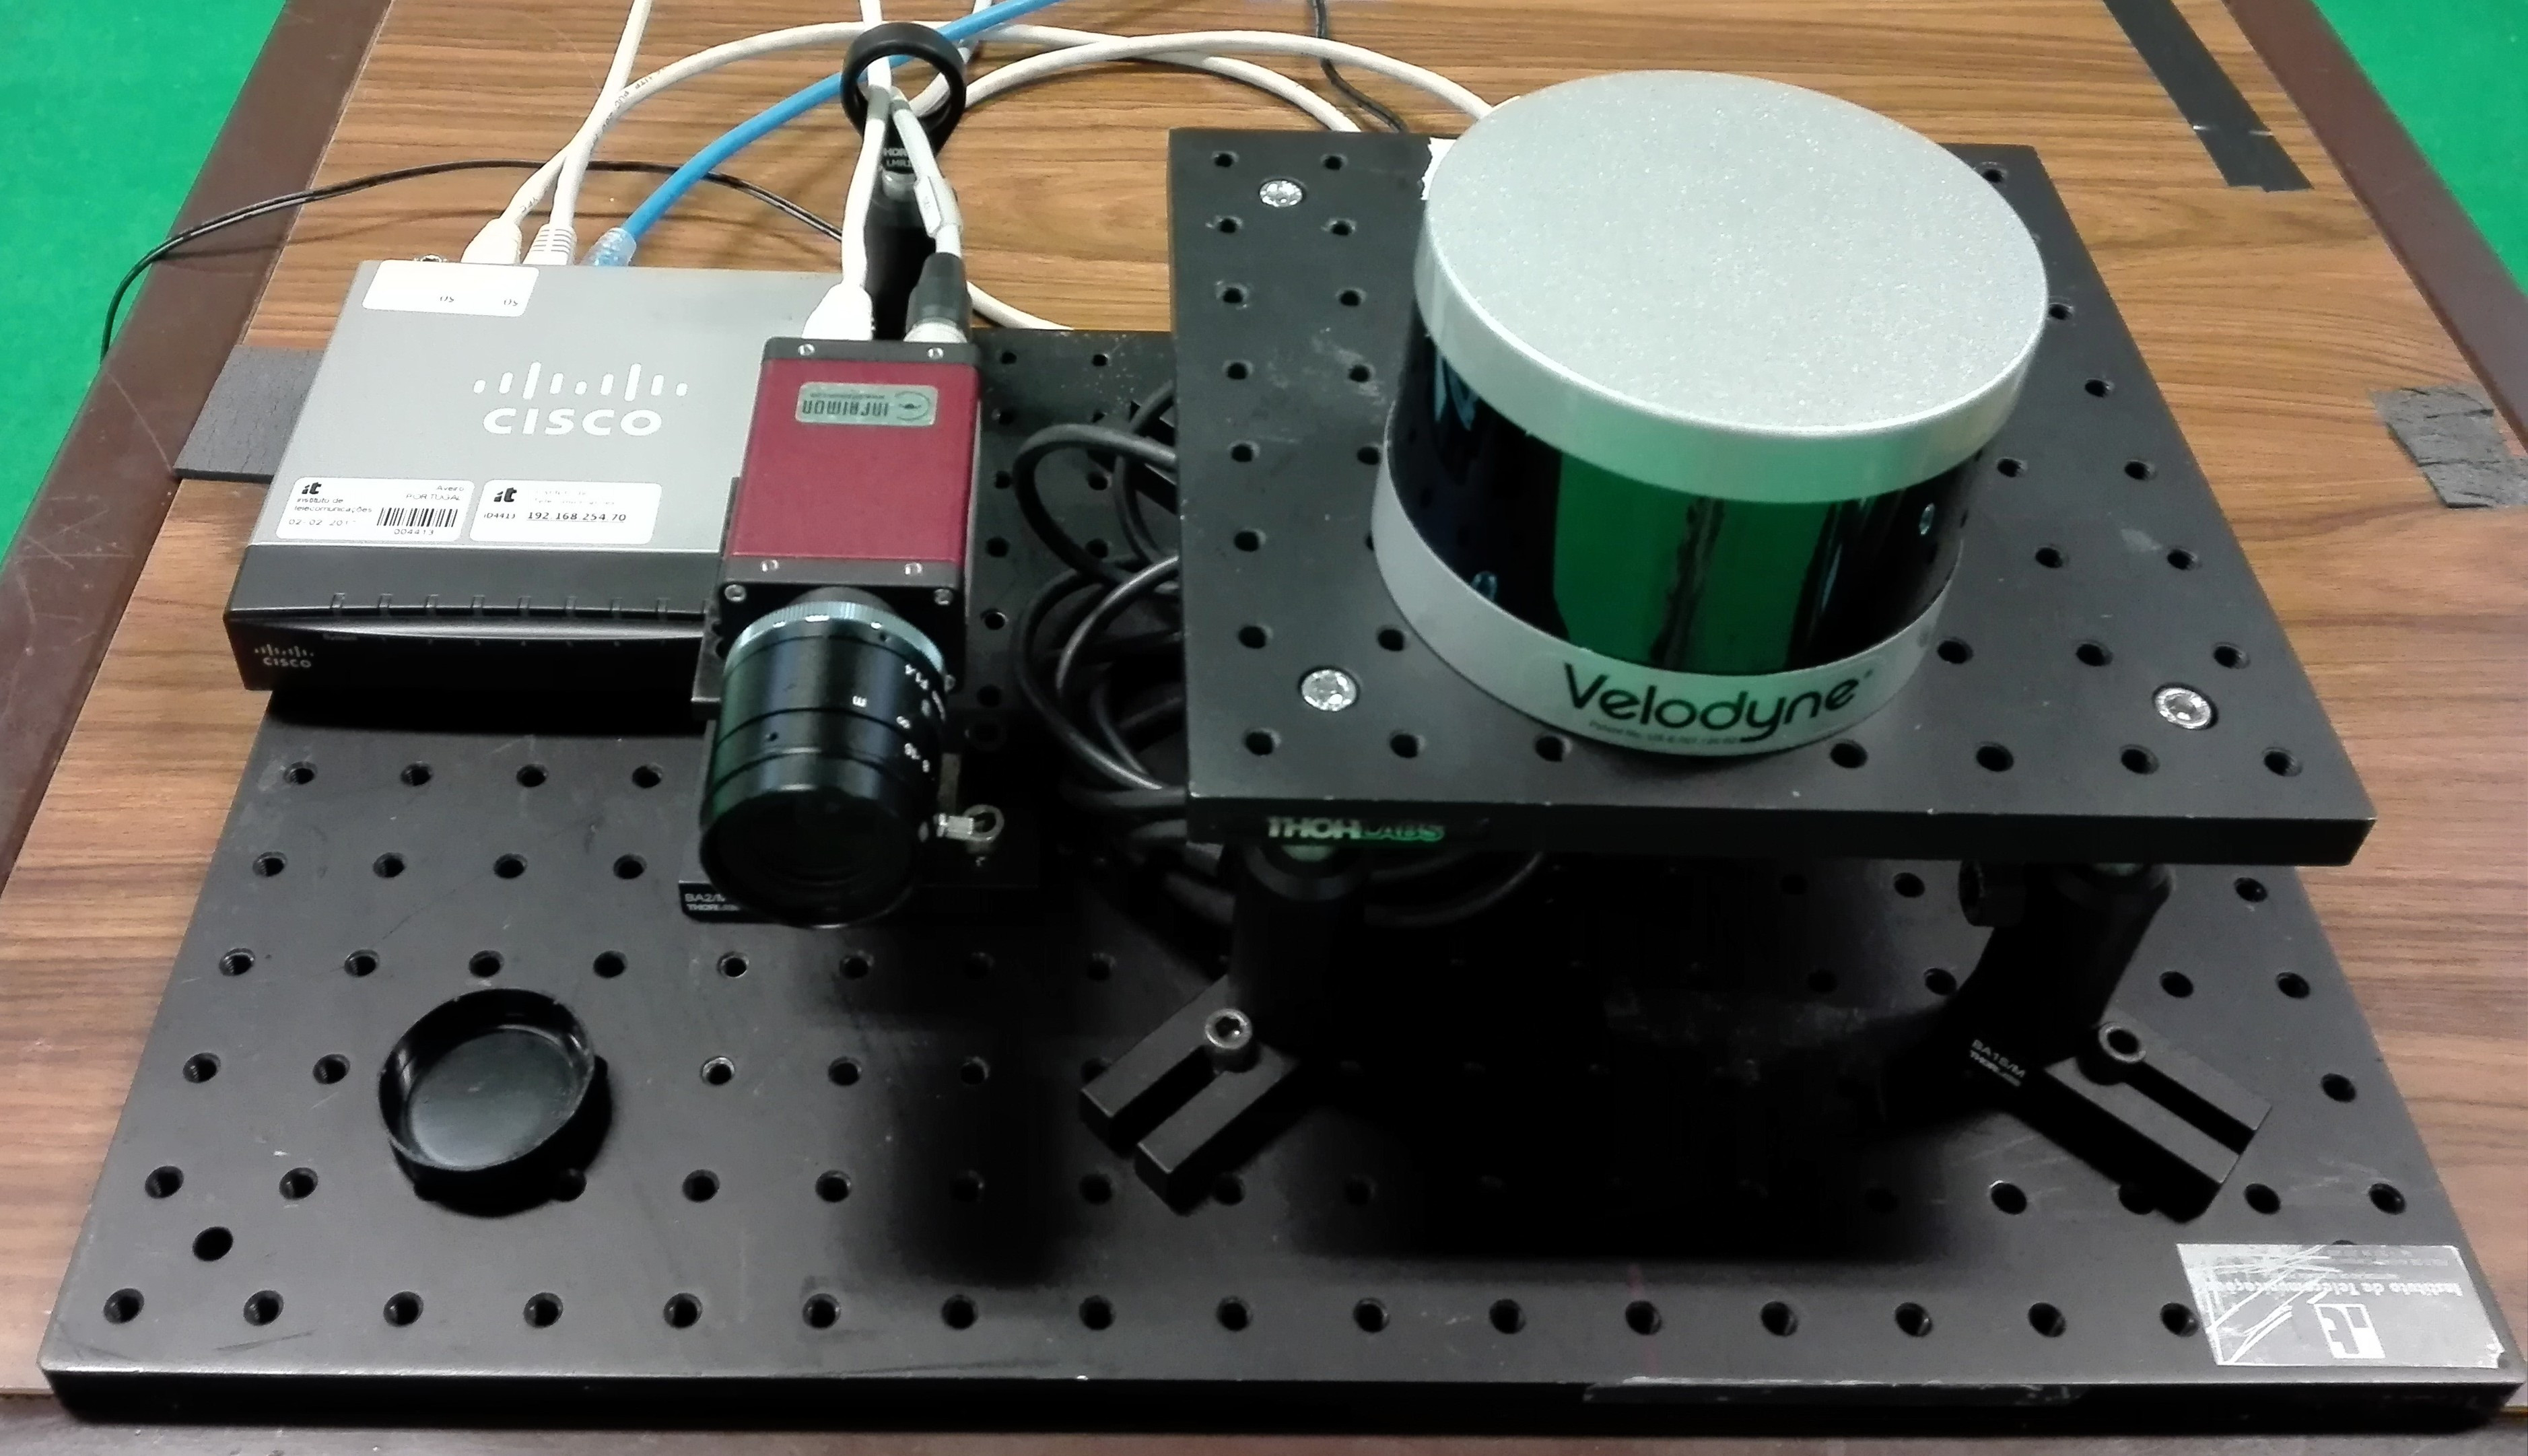
\includegraphics[width=\textwidth]{img/experimental-setup/table-setup-cambada-perspective.jpg}
		\caption{Experimental Setup viewed in perspective.}
		\label{fig:experimental-setup:perspective}
	\end{subfigure}
	\qquad
	\begin{subfigure}[c]{0.45\textwidth}
		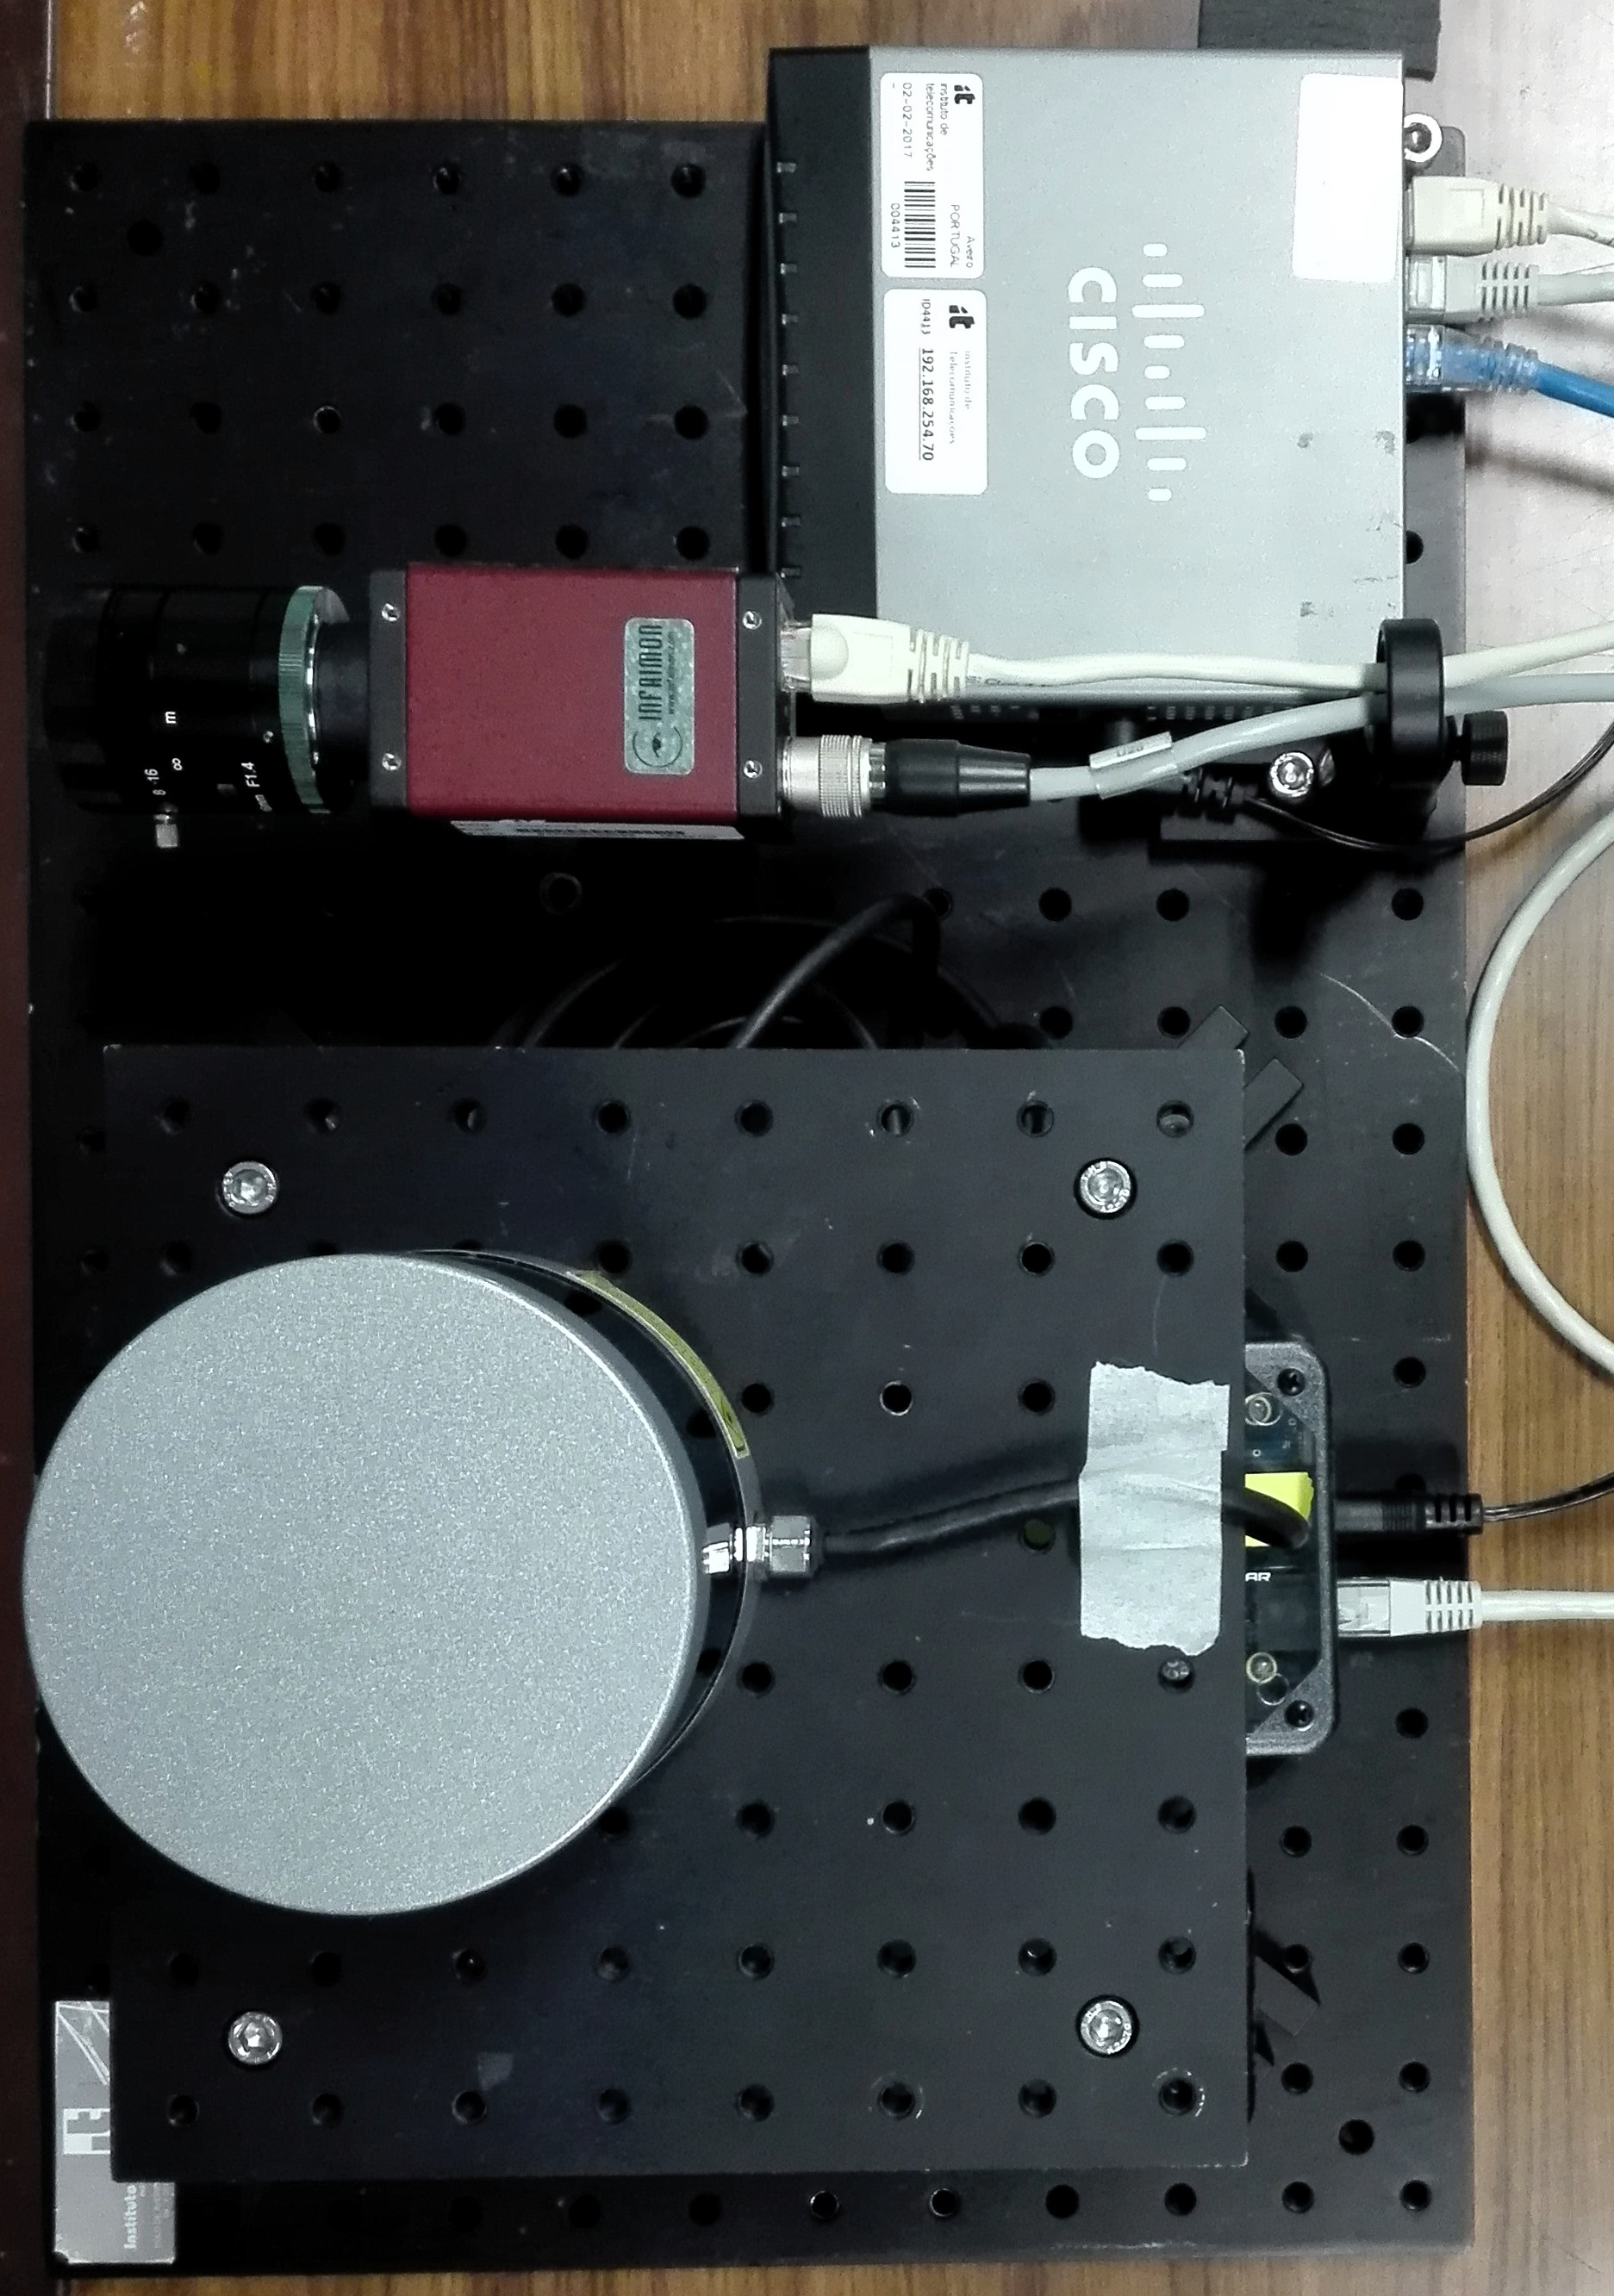
\includegraphics[width=0.65\textwidth, keepaspectratio, angle=90]{img/experimental-setup/table-setup-cambada-birds-eye.jpg}
		\caption{Experiemental Setup from a bird's eye view.}
		\label{fig:experimental-setup:birds-eye}
	\end{subfigure}
	\caption{Experimental Setup from a bird's eye view.}
	\label{fig:experimental-setup}
\end{figure}

\subsection{Camera and Lens}
The camera model used is an industrial 5 \ac{mp} RGB camera, from \ac{avt}  Manta G-504C. Camera lens is a 1" C-Mount format camera with lock from Thorlabs\cp, MVL16M1. The full camera specifications can be accessed on~\cite{MantaG504C} and the full lens specifications on~\cite{Thorlabs}. Relevant specifications of the camera and lens are summarized  on table~\ref{tab:camera-and-lens-specs}. 

\begin{table}[H]
	\renewcommand{\arraystretch}{1.2}
	\centering
	\begin{tabular}{@{}lp{7cm}l@{}}
		\toprule
		\multicolumn{2}{l}{Specification} & Value \\ \midrule
		\multicolumn{2}{l}{\emph{Camera}} & \\
		\phantom{a} & Full Resolution (width vs heigth) & $2452 \times 2056$   \\
									& Shutter mode & Global \\
									&	Maximum \ac{fps} at full resolution & $9.2$ \\ \midrule 
									\multicolumn{2}{l}{\emph{Lens}} \\
									&	Focal Length & $16$ mm \\
									&	Max aperture & $f/1.4$ \\
									&	Minimum Object Distance & $300$ mm  \\
									& \acs{adc}\footnotemark bit depth & $12$ bit \\
		\bottomrule
	\end{tabular}
	\caption{Relevant specifications for \ac{avt} Manta G504C RGB camera (from~\cite{MantaG504C})  and MVL16M1 Thorlabs\cp~lens (from~\cite{Thorlabs}).}
	\label{tab:camera-and-lens-specs}
\end{table}

\footnotetext{\acs{adc} stands for \acl{adc}}

To power the Manta G-504C, a laboratory power source must be used. Manta consumes $3.9 W$~\cite{MantaG504C} while operating, accepting an input voltage between $8$ and $30$ $V_{DC}$. The power source used was set to  $12 V_{DC}$ and the current output was $\approx 0.33A$. Voltage and current were measured during all tests, and summarized qualitative results are presented on table~\ref{tab:manta-power}. The power cable provided is an U20 \ac{udp} cable with a HIROSE HR10A-10P-12S female connector. Since the mapping from the 8 pins \ac{udp} cable to the 12 pin connector was not available, a continuity test was made between the expected pinout of the power cable (for more details, see~\cite{AVTCables}) and its the real pinout. The results can be consulted in~\nameref{sec:appendix-b}, on table~\ref{tab:manta-power-cable-pinout}.

	
\begin{table}[H]
	\centering
	\renewcommand{\arraystretch}{1.2}
	\renewcommand{\tabcolsep}{0.45cm}
	\begin{tabular}{@{}llll@{}}
		\toprule
					  & Minimum & Maximum & Median Value \\ \midrule
		Current ($mA$) & $298 \pm 1$ & $330\pm 1$ & $312 \pm 1$ \\
		Voltage ($V$)  & $12.00\pm 0.07 $ & $12.18\pm 0.07$ & $12.08\pm0.07$ \\
		\bottomrule
	\end{tabular}
	\centering
	\label{tab:manta-power}
	\caption{Voltage and Current measurements during Manta AVT G-504C operation. Minimum and Maximum values were registered, along with the median. }
\end{table}



\subsection{\ac{tof} \ac{lidar}}
The \ac{tof} \ac{lidar} used is a Velodyne VLP-16\texttrademark, a 16 beam \ac{lidar} that operates with a wavelength of 903nm. VLP-16 supports various measurements modes based on the return pulse (Strongest, Last, Dual) and can be connected to a \ac{gps} for geopositioning and synchronize their time frames. It also supports several rotation velocities, from 300 to 1200 \ac{rpm}, which result in different angular steps and point cloud refresh rate. The full specifications can be acessed on~\cite{VLP16} and the relevant specifications for this work are summarized on table~\ref{tab:vlp16-specs}.

\begin{table}[H]
	\renewcommand{\arraystretch}{1.2}
	\centering
	\begin{tabular}{@{}p{8.3cm}l@{}}
		\toprule
		Specification & Value \\ \midrule
		Wavelength    & 903nm \\
		Motor \acs{rpm} & $600 \pm 3$ \\
		Angular step & 0.2º \\
		Vertical \ac{fov} & 30º \\
		Horizontal \ac{fov} & 360º \\
		Maximum Scanning Distance & 100m \\
		Max Error & $2 cm$ \\
		\bottomrule
	\end{tabular}
	\caption{Velodyne VLP-16 relevant specifications. Source~\cite{VLP16}.}
	\label{tab:vlp16-specs}
\end{table}


\subsection{Setup Connection and Risk of Interference}
Both Velodyne VLP-16 and \ac{avt} Manta G-504C operate over Gigabit Ethernet. Therefore, a Gigabit switch is required to connect all the equipment to a single computer using a single Ethernet port. The switch used was Cisco SG200-08, a 8-Port Gigabit Smart Switch. 

The switch was configured so that every port was on the same \ac{vlan}, ensuring packets were accessible on the computer. An alternative was to redirect the packets from each sensor to the computer network and filter the packets from the computer to the sensor by putting them on separated networks. However, Since no bandwidth constraints existed and packet delay or loss ocurred, the solution chosen was the former, due to its simplicity. 

For each device a fixed \ac{ip} address as attributed, following the intructions on their datasheet~\cite{VLP16, MantaVision2013}. The \acp{ip} addresses can be consulted on table~\ref{tab:experimental-setup-ip}.

\begin{table}[H]
	\renewcommand{\arraystretch}{1.2}
	\centering
	\begin{tabular}{@{}lcc@{}}
		\toprule
		Device          & \ac{ip} Adress & Subnet Mask\\ \midrule
		Computer        & 192.168.10.77  & 255.255.255.0 \\
		Manta G-504C    & 192.168.10.1   & 255.255.255.0 \\
		Velodyne VLP-16 & 192.168.10.201 & 255.255.255.0 \\
		\bottomrule
	\end{tabular}
	\label{tab:experimental-setup-ip}
	\caption{\acp{ip} and subnet masks for the devices connected on the experimental setup.}
\end{table}

No significant interference is expected between the camera and the \ac{lidar}. Despite the camera lens having a tranmission coefficient of $66\%$ at $900 nm$~\cite{Thorlabs}, Sony ICX655, the camera sensor for the \ac{avt} Manta G-504C, only was a Quantum Efficiency of $\approx 6\%$~\cite{MantaG504C}. To test this hypotheses, the experimental setup was switched on in a Dark Room without any light sources and the data was visualized. No interference could be seen from the \ac{lidar} infrared beams when looking on the camera image feed. Therefore, no further research on \ac{lidar} to camera interference were carried. 


%\begin{figure}[H]
%	\centering
%	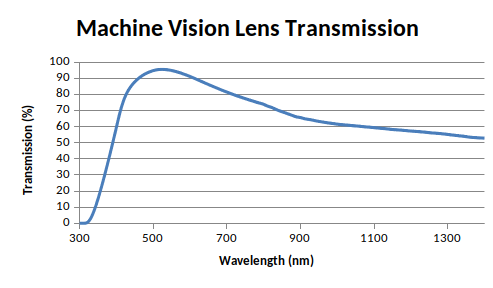
\includegraphics[width=0.6\textwidth]{img/experimental-setup/lens-transmission.png}
%	\caption{Transmission of the MVL16M1 lens in relation the light wavelength. Source~\cite{Thorlabs}}
%	\label{fig:lens-transmission}
%\end{figure}



\section{Camera Intrinsic Calibration}
The act of calibrating a camera consists on determining its intrinsic parameters, as detailed in subsection~\ref{subsec:sota:camera-intrinisc-calibration}. This can be done by taking different images with a know pattern fully visible on the camera \ac{fov}, changing its rotation an translation relating tho the camera.

The calibration procedure undertaken uses a chessboard of $13 \times 9$ squares, with each square having an edge length of $44.0mm$. The chessboard used can be seen on figure~\ref{fig:chessboard}. It was laser printed on paper and then glued to a plywood board.

\begin{figure}[H]
	\centering
	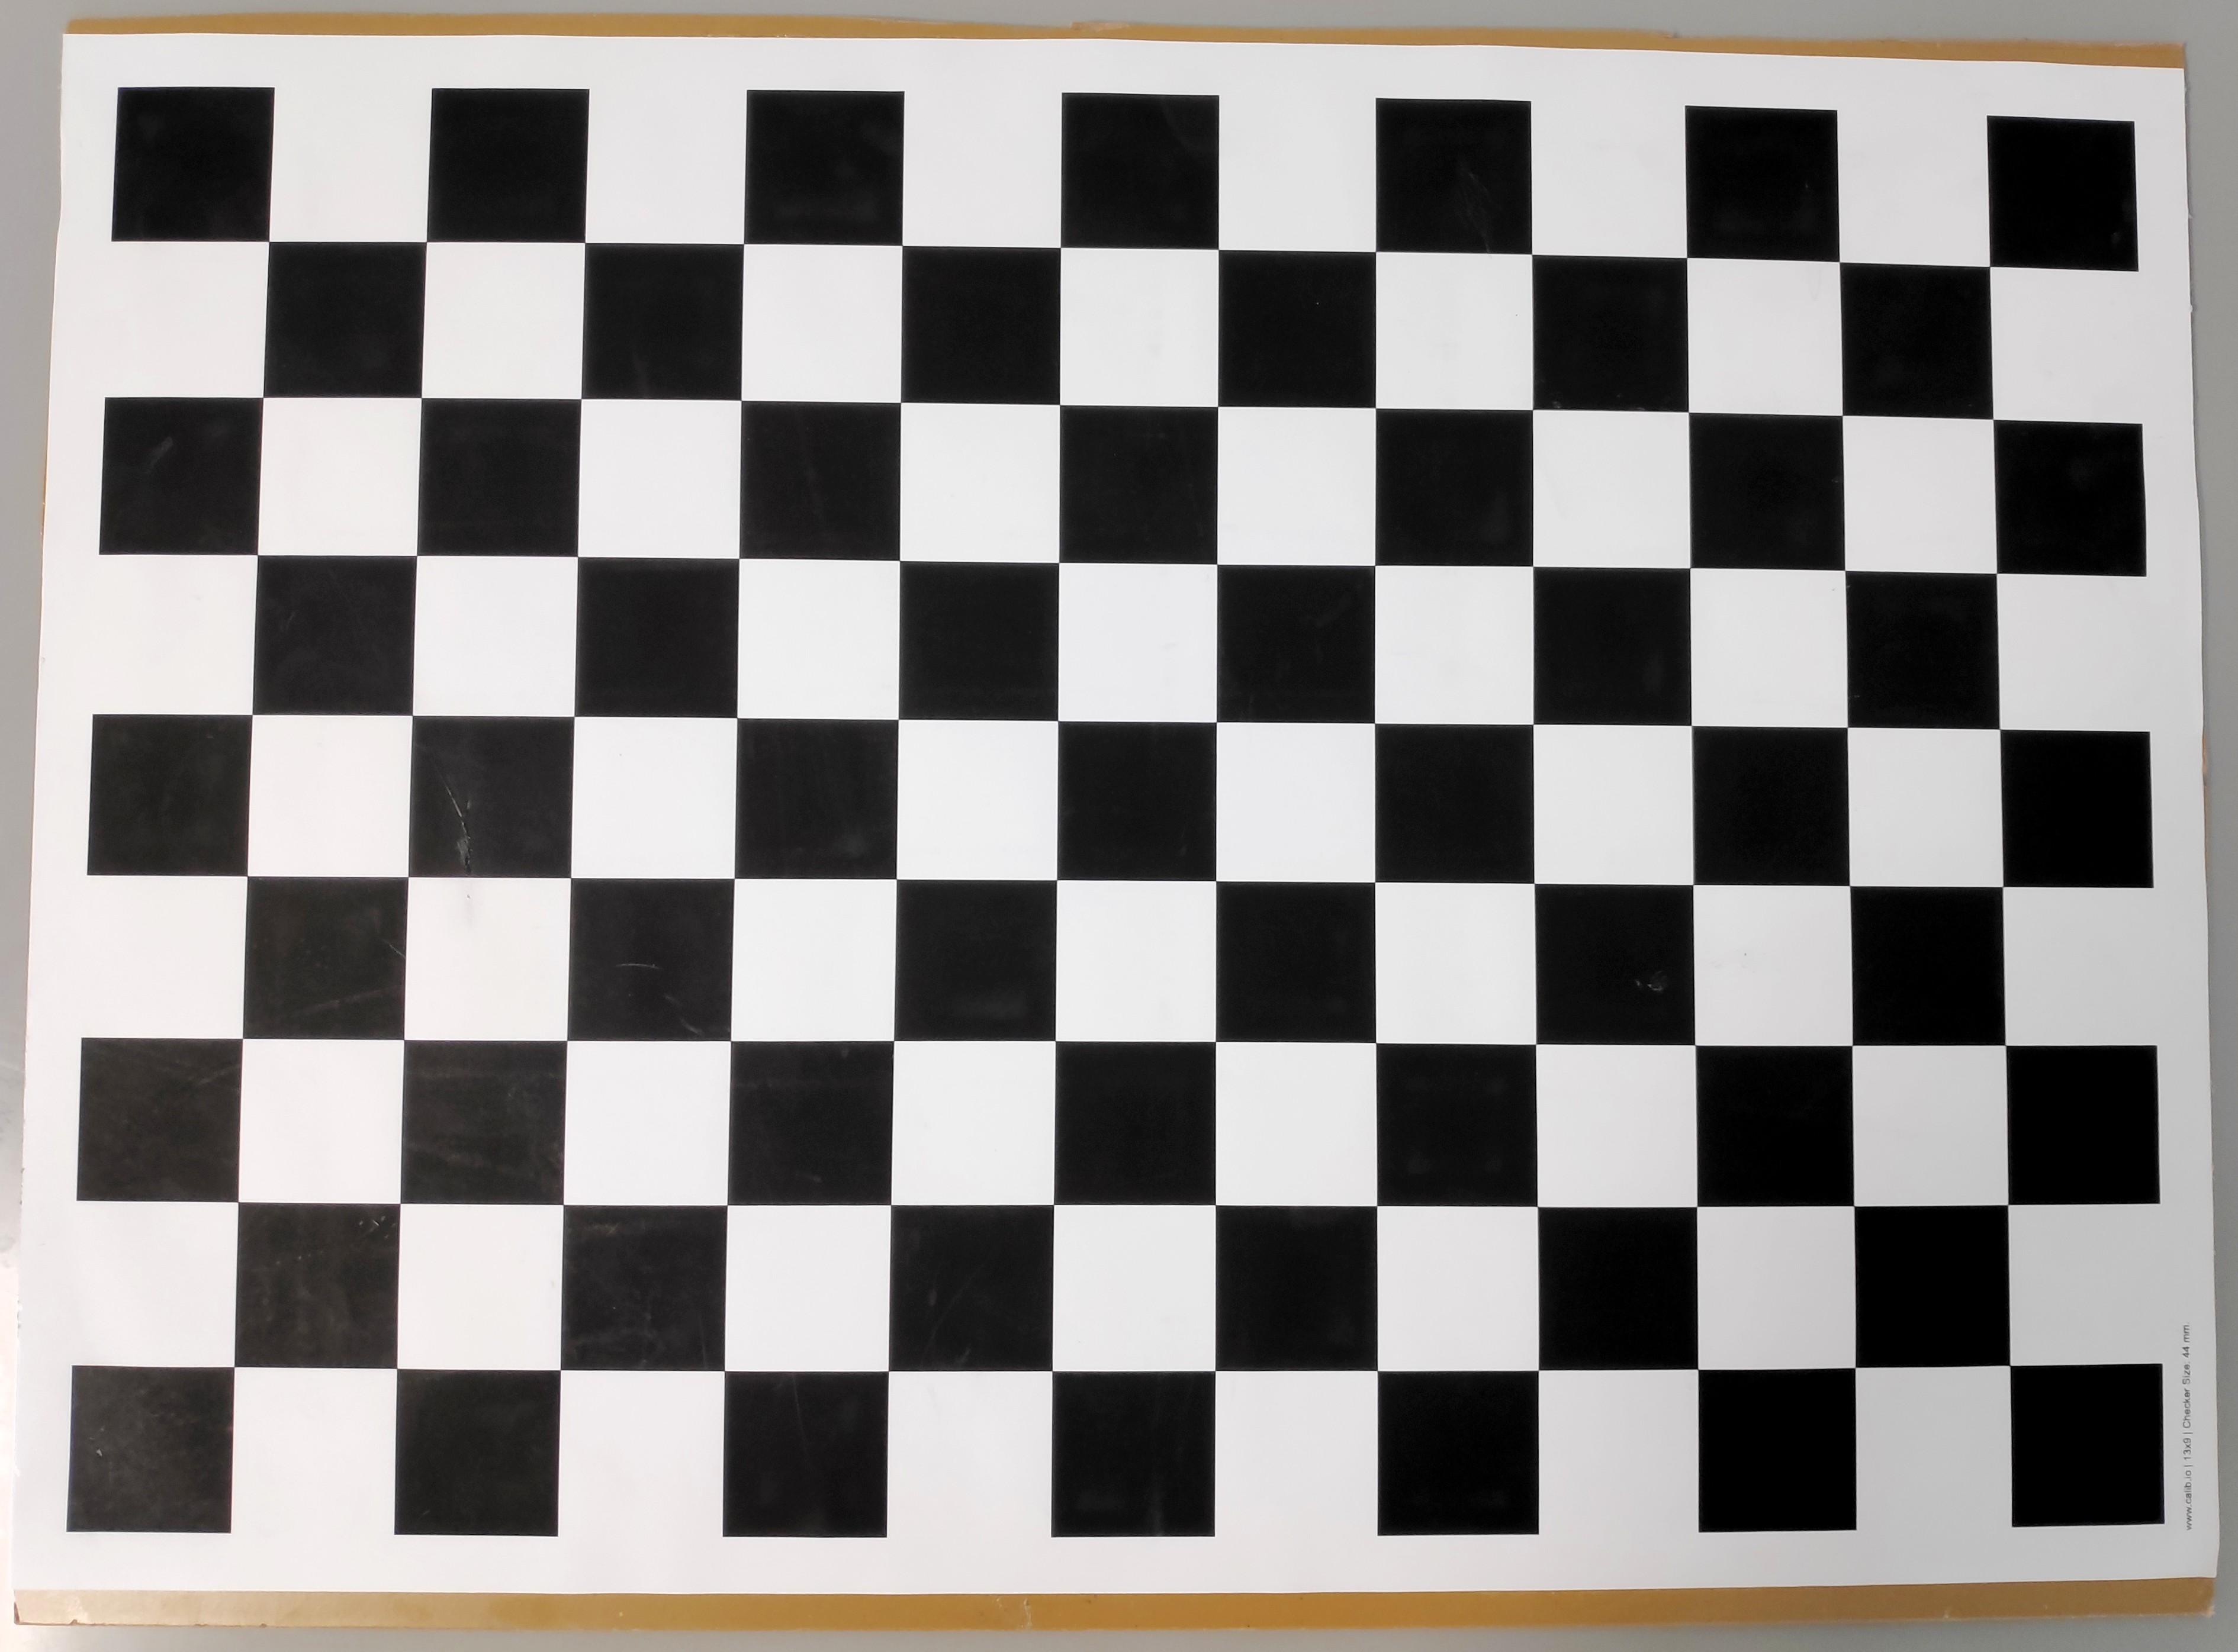
\includegraphics[width=0.5\textwidth]{img/experimental-setup/chessboard.jpg}
	\caption{Chessboard used during camera calibration procedures. The chessboard was laser printed on A2 paper size, in real size, that was then glued to a plywood board.}
	\label{fig:chessboard}
\end{figure}

Calibrating the camera requires that the calibration object to be focused. Therefore, before any proper calibration can be made, focus theory and procedure are layed out on the next sub-section,~\ref{subsec:calibration:camera-focus}.


\subsection{Camera Focus and \acl{dof}}
\label{subsec:calibration:camera-focus}
Focusing a camera can only be attained for an exact distance from the camera~\cite{Merklinger1993, Photopillers}, measured perpendicularly to the plane of focus, which is the plane containing the \ac{cmos} or \ac{ccd} chip. Therefore, on every image, there is a plane of focus and what actually ``looks focused'' is really just ``acceptably sharp focus'', since precise focus is only possible to an exact distance, and not for an entire tridimensional object.

``Acceptably sharp focus'' means that a point in the real world would not result in a point on the image (as happens in precise focus), but in a blurred spot that is circular (due to the form of the aperture)\cite{Photopillers}. However, if the size of blur is small enough, little to no differences can be perceived and the image is considered to be focused\cite{Photopillers}. The maximum size at which this blur is not noticed by the viewer (given a specific sensor size, dimension of the viewed photo, viewing distance and acuity of the viewer) is called the \ac{coc}\cite{Photopillers, Merklinger1993}.

The first step in focusing an image requires the calculation of the hyperfocal distance, $H$: the distance at which the camera is focused to ensure objects from half of this distance to the infinity are in an ``acceptably sharp focus'' (refer to as just focus, from now on). This distance can be calculated using the equation~\ref{eq:hyperfocal_distance}, below, where $f$ is the focal length, $F_N$ is the F-number and $c$ the \ac{coc} limit. Hyperfocal near limit is defined as $H_{near} = \rfrac{H}{2}$.

\begin{equation}
	\label{eq:hyperfocal_distance}
	H = \frac{f^2}{F_Nc} + f \approx \frac{f^2}{F_Nc} 
\end{equation}

Known the hyperfocal distance, the \acf{dof} can be calculated. \ac{dof} is measured in meters and is obtained by subtracting the farthest and nearest distances at which an object is focused (see equation~\ref{eq:dof}), indicating the distance between this two points\cite{Photopillers, Merklinger1993, mvg_book}. The nearest and farthest points can be calculated using the equations~\ref{eq:dof-near} and~\ref{eq:dof-far}, respectively.

\begin{subequations}
	\label{eq:dof_all}
	\begin{align}
		DoF & = DoF_{far} - DoF_{near} \label{eq:dof} \\
		DoF_{far} & = \frac{H\times d}{H - (d - f)} \label{eq:dof-far} \\
		DoF_{near} & = \frac{H\times d}{H + (d - f))} \label{eq:dof-near} 
	\end{align}
\end{subequations}

Using equations~\ref{eq:dof_all} is possible to select a desired \acl{dof} for an image that guarantees that all the objects of interest are focused. Taking in consideration that smaller apertures (bigger F-numbers) will increase the exposition time\cite{Merklinger1993}, a target distance can be selected with the guarantee that all the objects from the near \ac{dof} point to the far \ac{dof} will be sharp.

Rewriting the equation~\ref{eq:dof-near} to calculate the object's distance, giving the mininum distance at the objects must be focused, one gets the equation~\ref{eq:dof-subject-distance}.

\begin{equation}
	\label{eq:dof-subject-distance}
	d = \frac{(H - f) \cdot DoF_{near}}{H - DoF_{near}}
\end{equation}


\subsection{Camera Calibration Procedure}
For calibration, the \ac{opencv} standard algorithms are used~\cite{opencv_doc}, such as \emph{calibrateCamera}, \emph{solvePnP} and \emph{findChessboardCorners}. This algorithms, their interconnections and a \ac{gui} for performing calibration are wrapped on a \ac{ros} package, \emph{camera\_calibration} from the \emph{image\_pipeline} metapackage~\cite{cameraCalibrationRos}, which is used.

For calibration, around 50 unique photos are taked for each setup. These images are converted to grayscale, the chessboard corners are detected and the camera intrinsic parameters are computed by the ROS package. A subset of the calibration images is presented on figure~\ref{fig:camera-calibration-images}.

\begin{figure}[h]
	\centering
	\begin{subfigure}[c]{0.30\textwidth}
		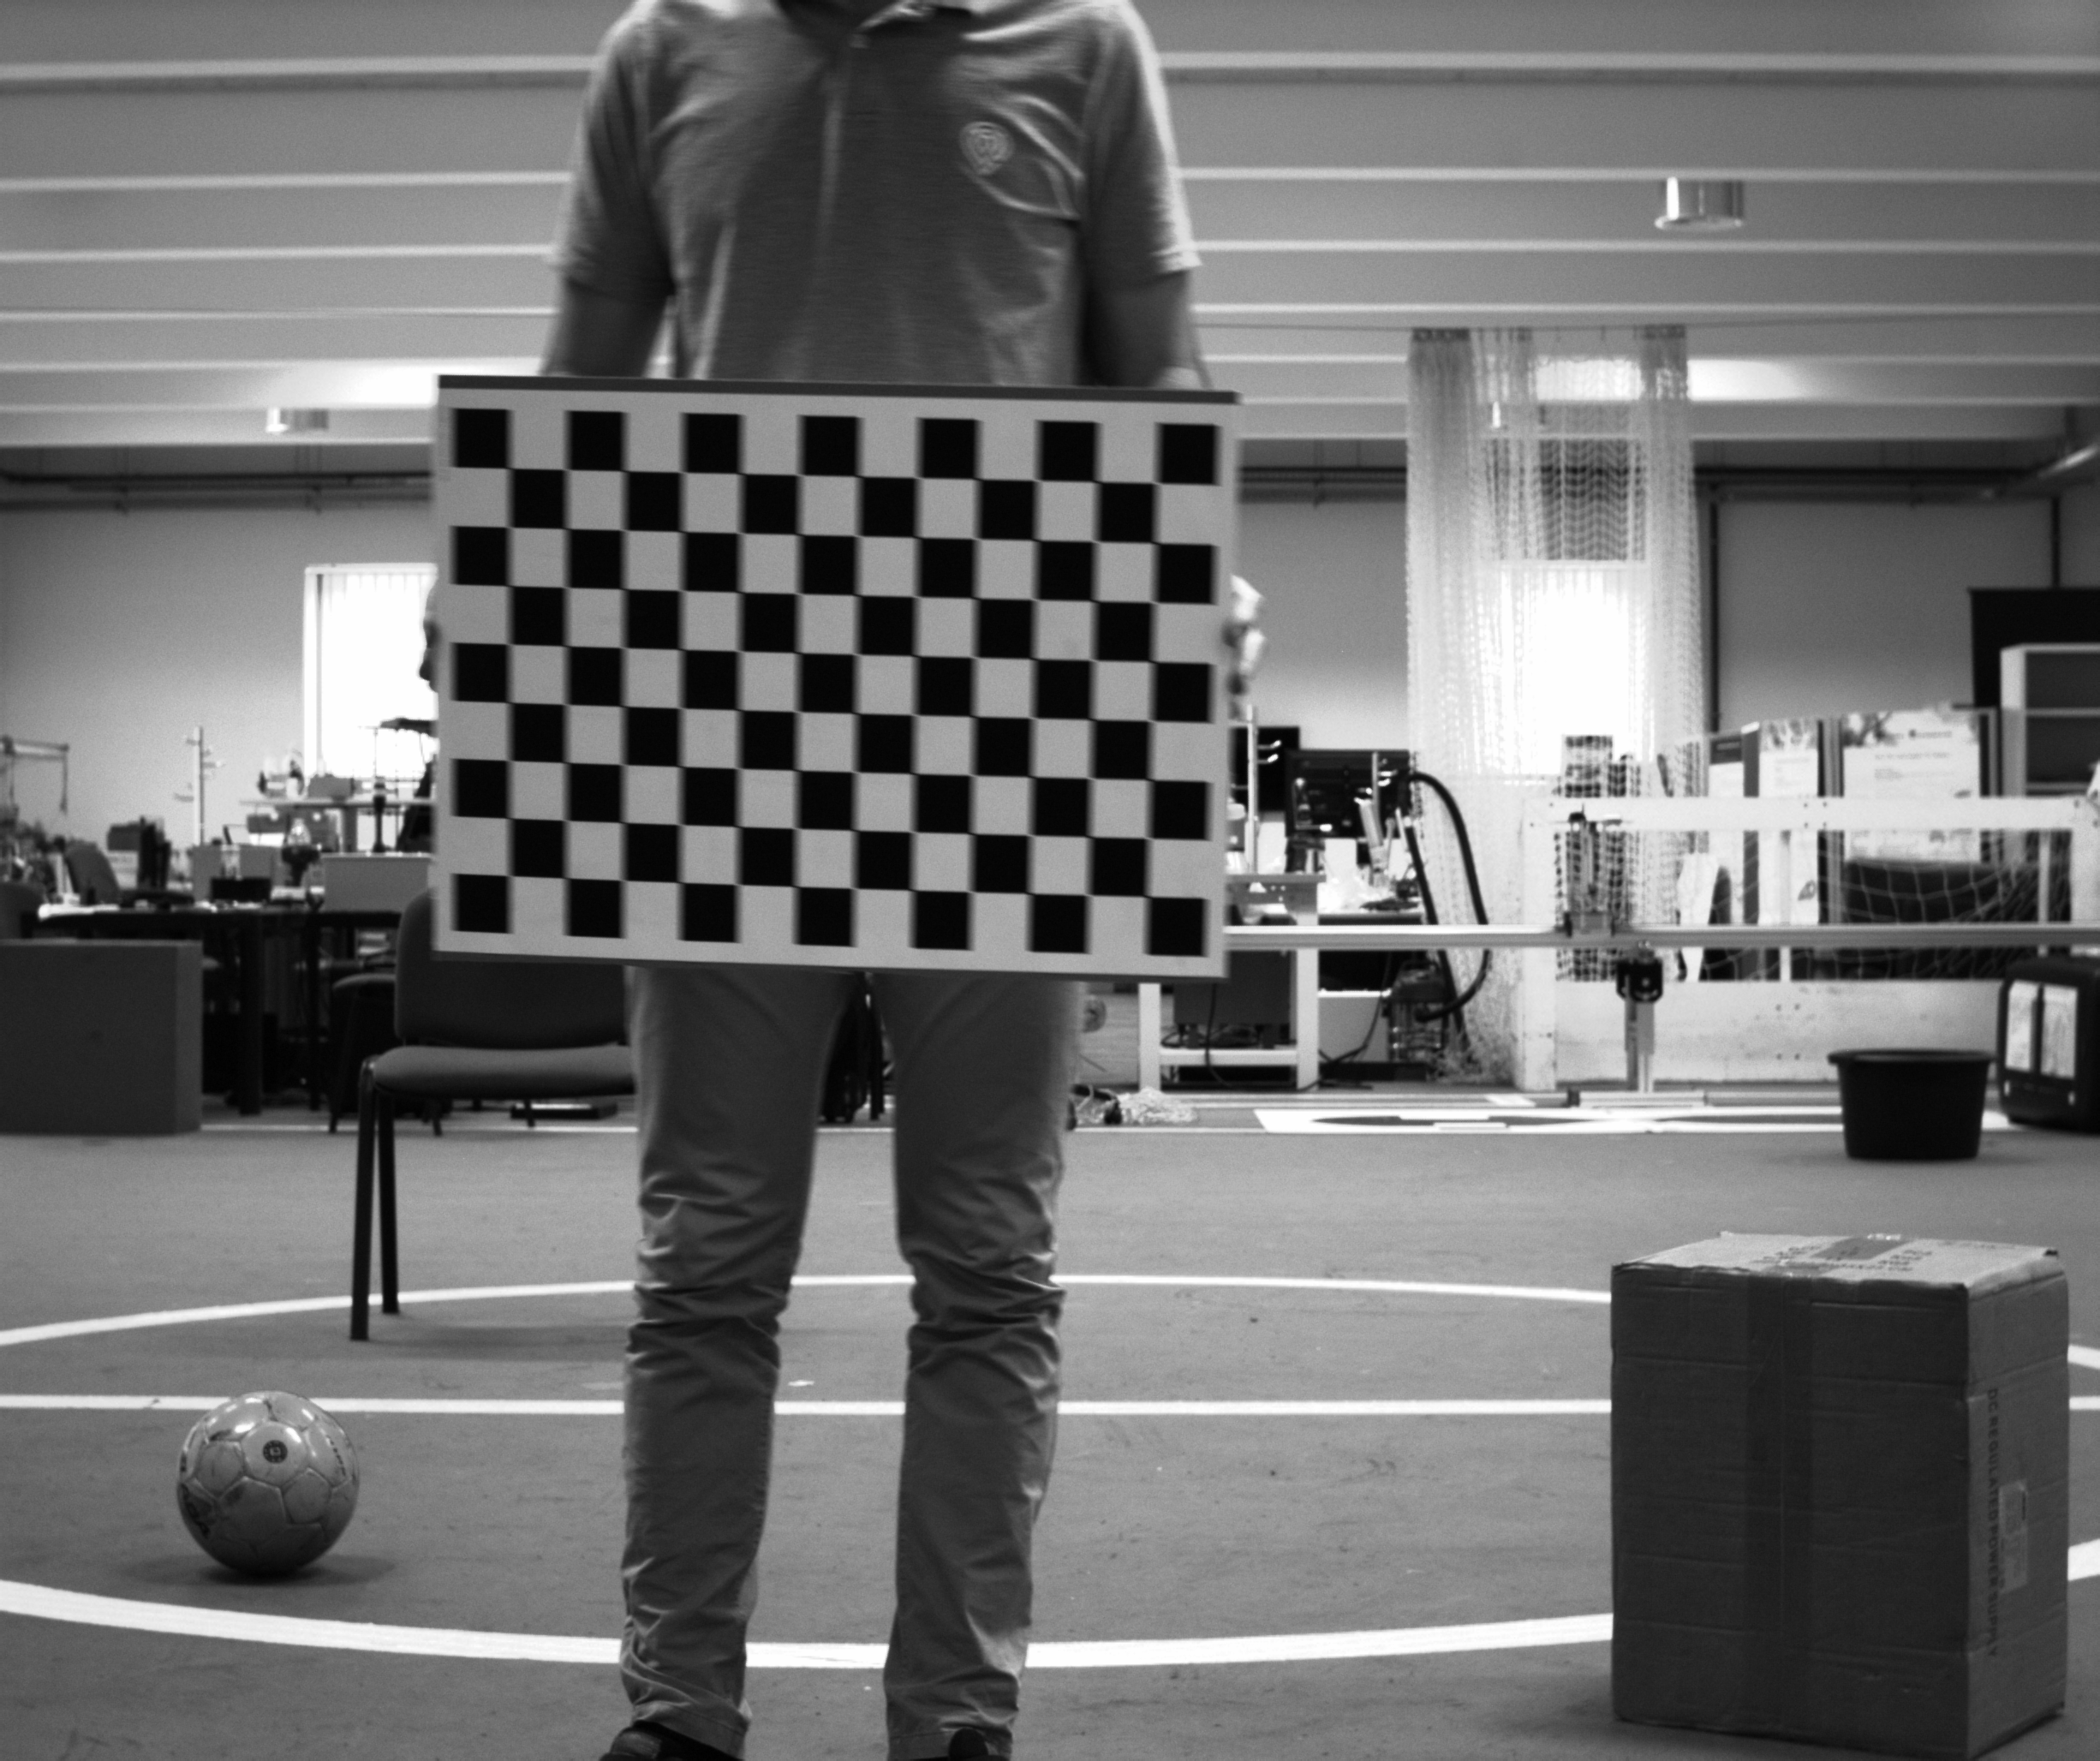
\includegraphics[width=0.9\textwidth]{img/camera-calibration/left-0001.png}
	\end{subfigure}
	\begin{subfigure}[c]{0.30\textwidth}
		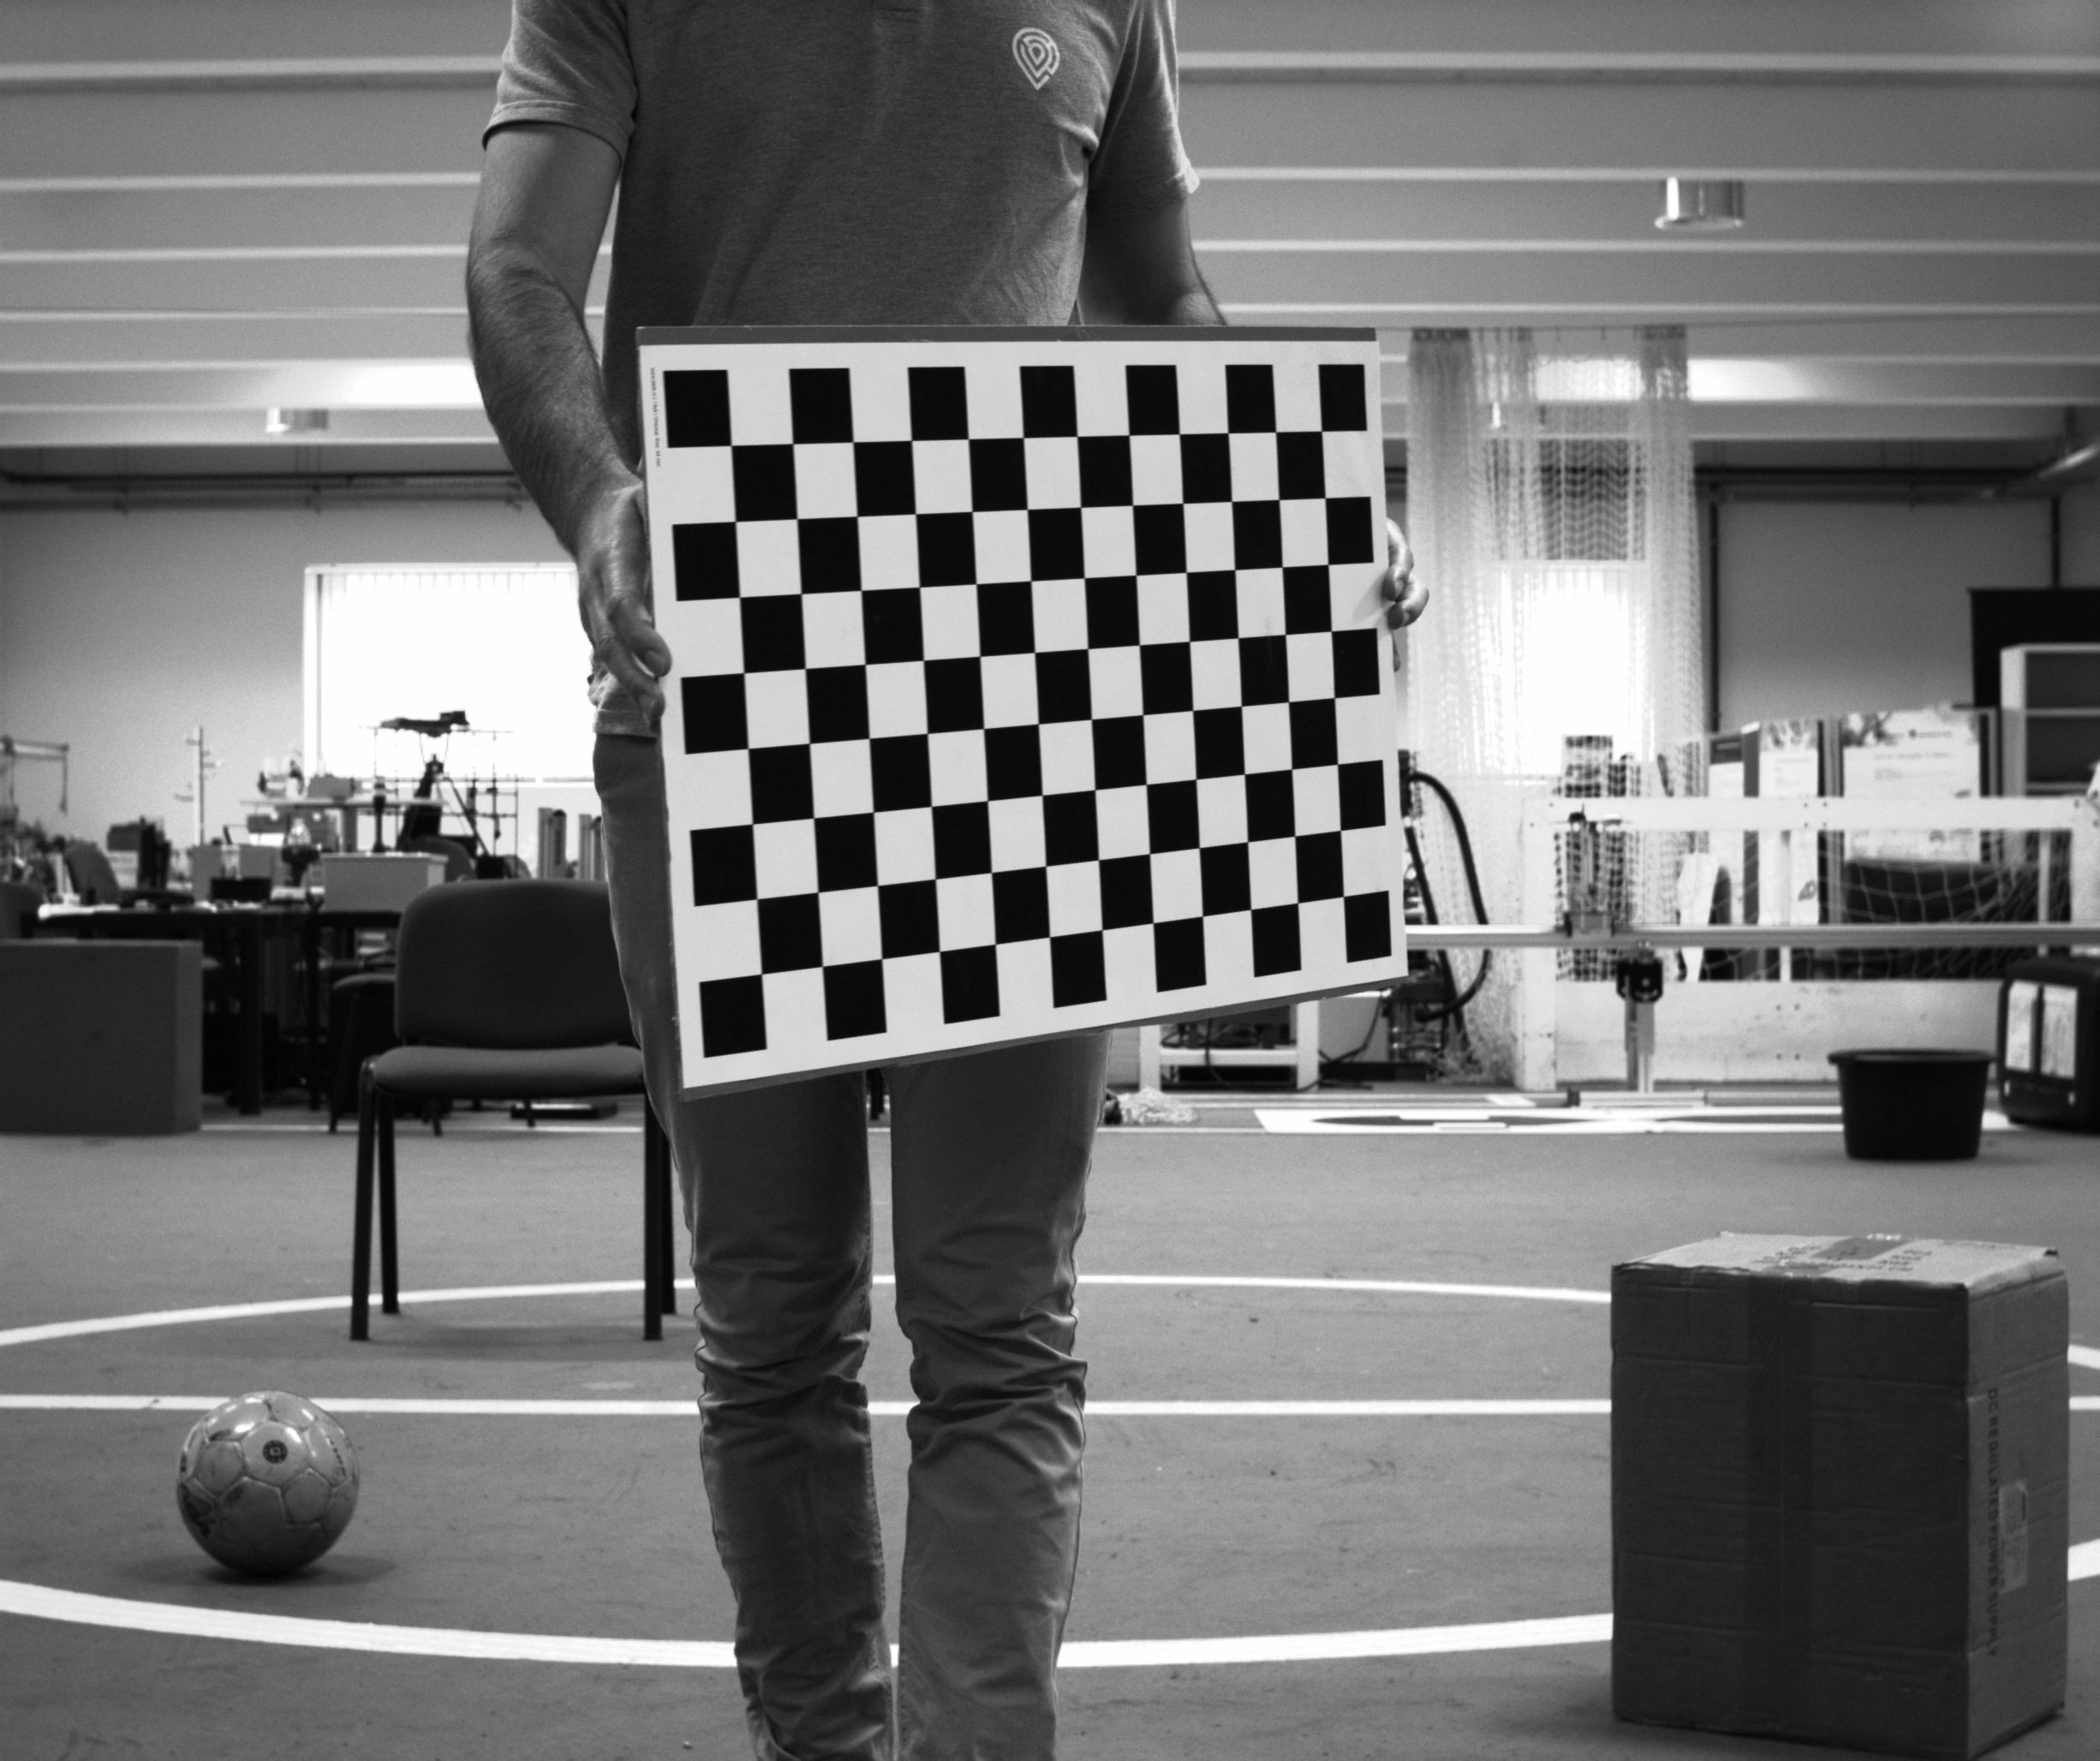
\includegraphics[width=0.9\textwidth]{img/camera-calibration/left-0005.png}
	\end{subfigure}
	\begin{subfigure}[c]{0.30\textwidth}
		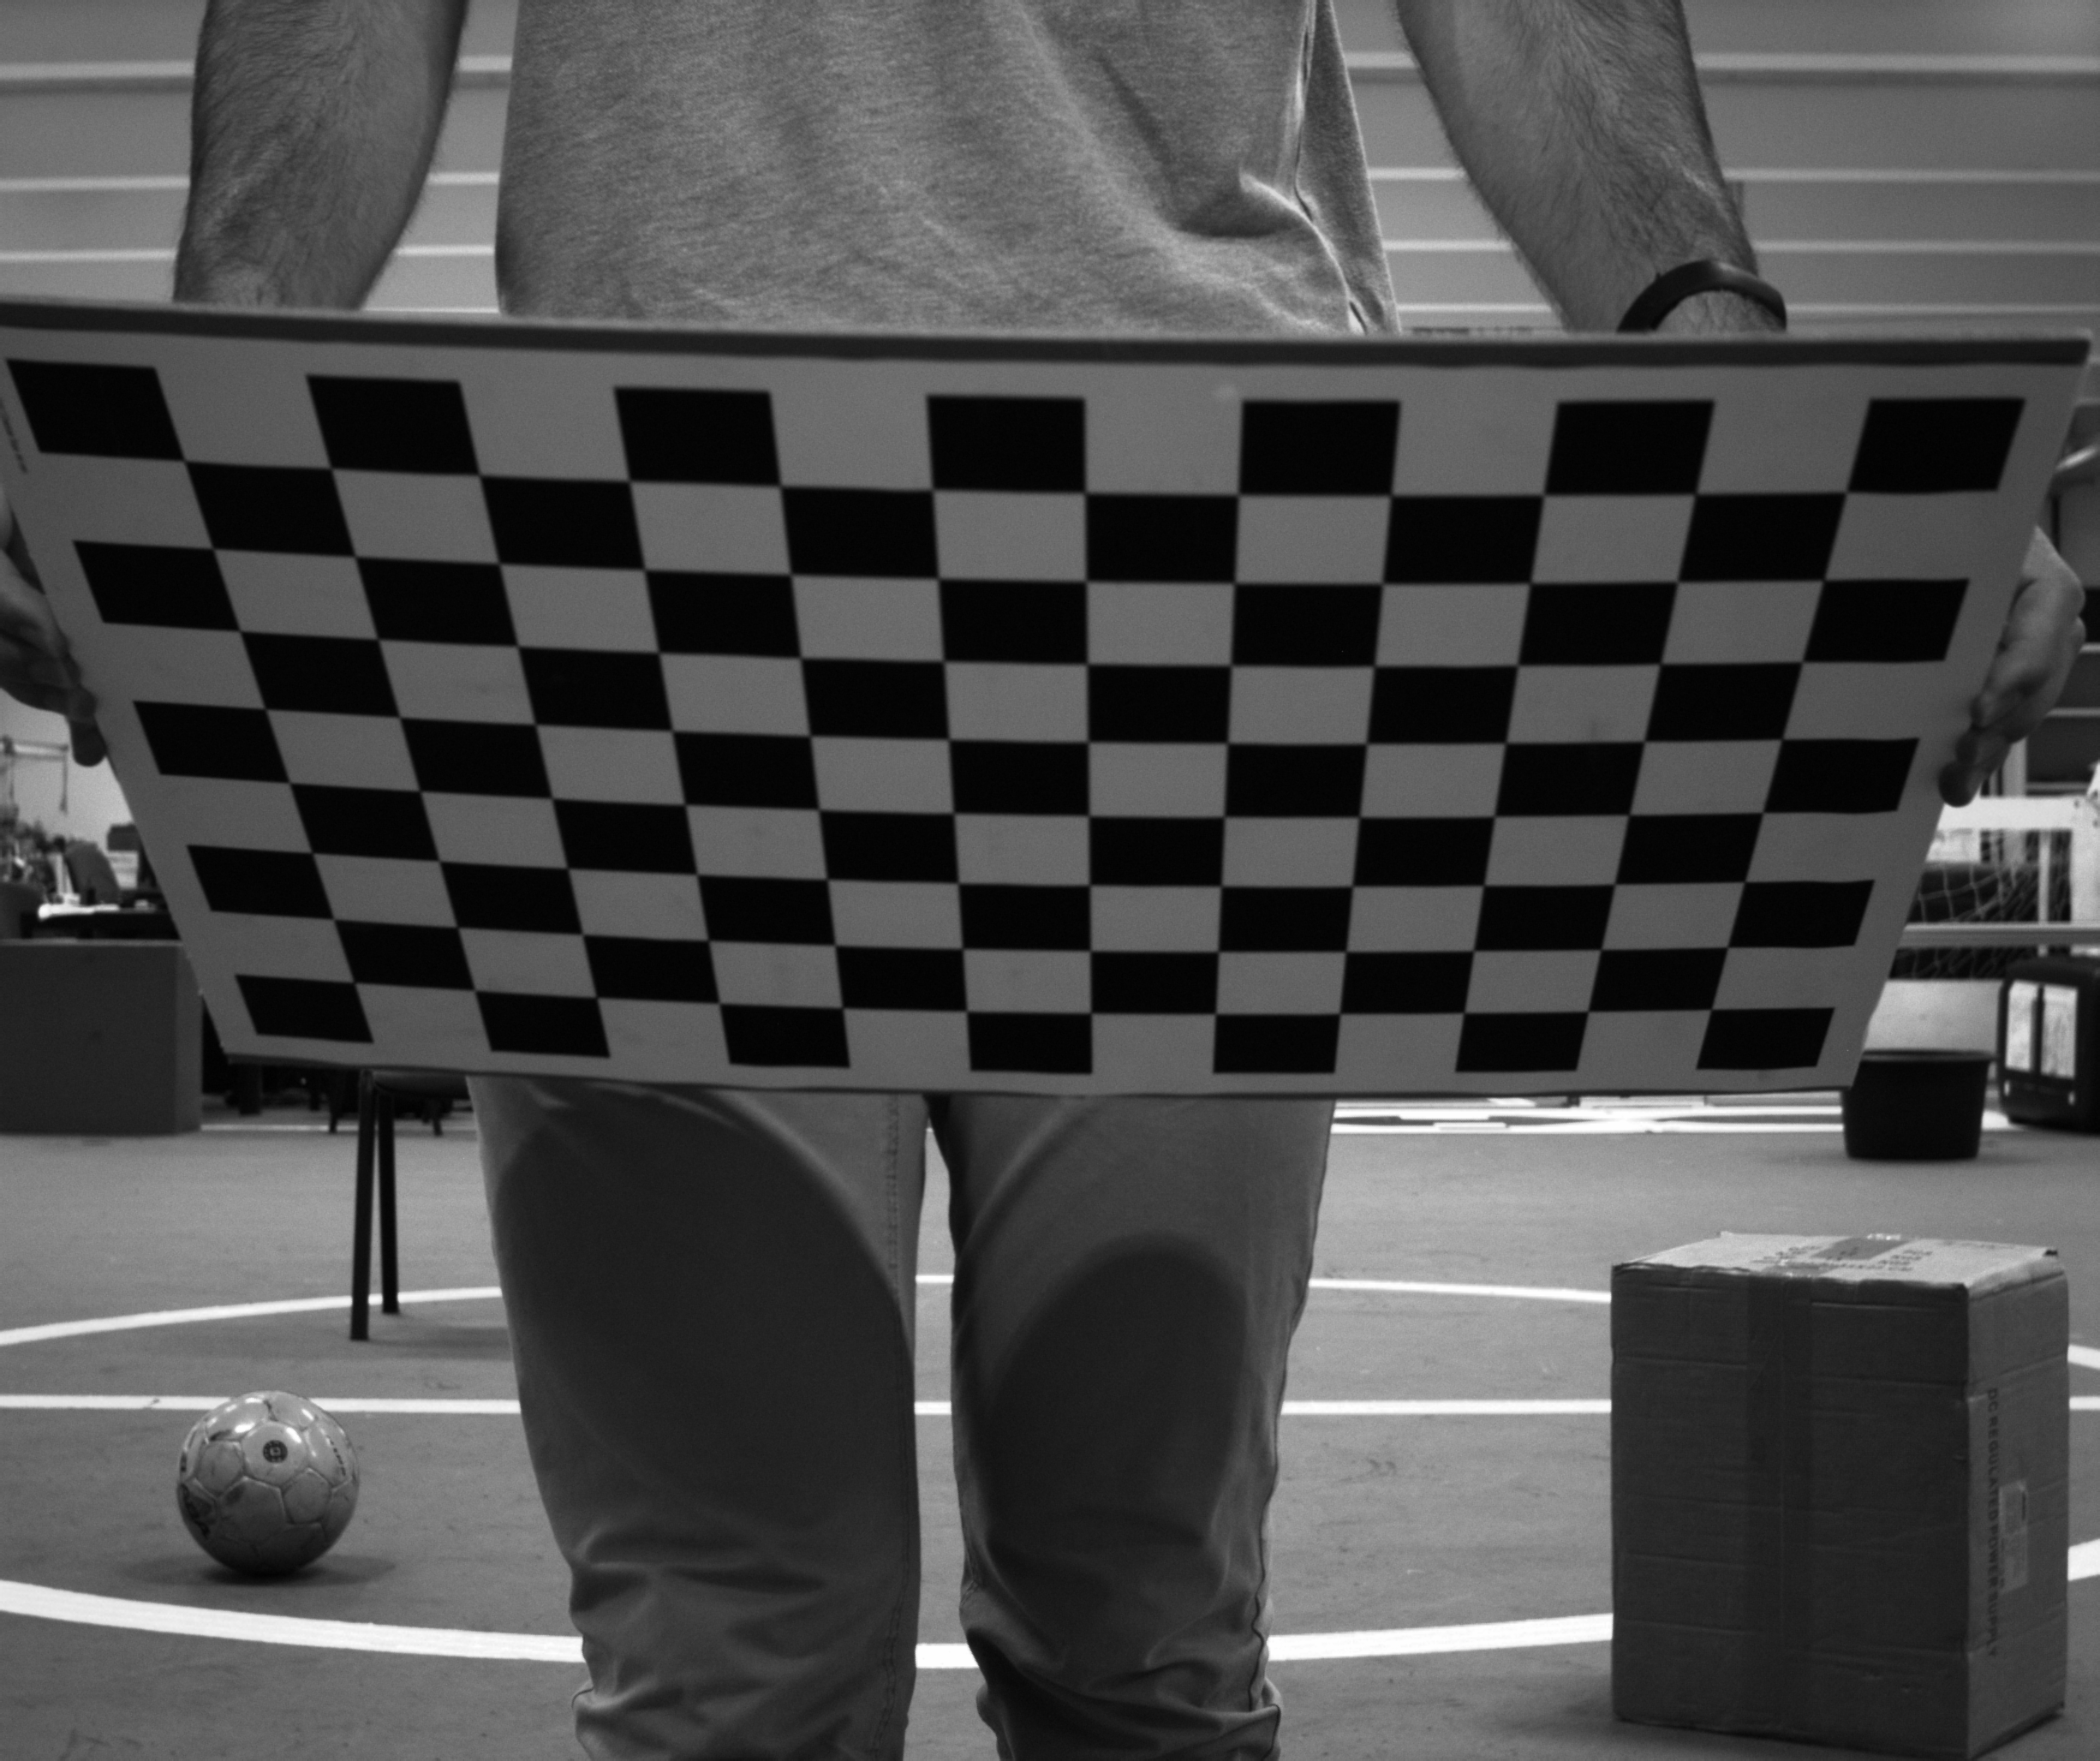
\includegraphics[width=0.9\textwidth]{img/camera-calibration/left-0022.png}
	\end{subfigure}
	\\ 
	\vspace{5mm}
	\begin{subfigure}[c]{0.30\textwidth}
		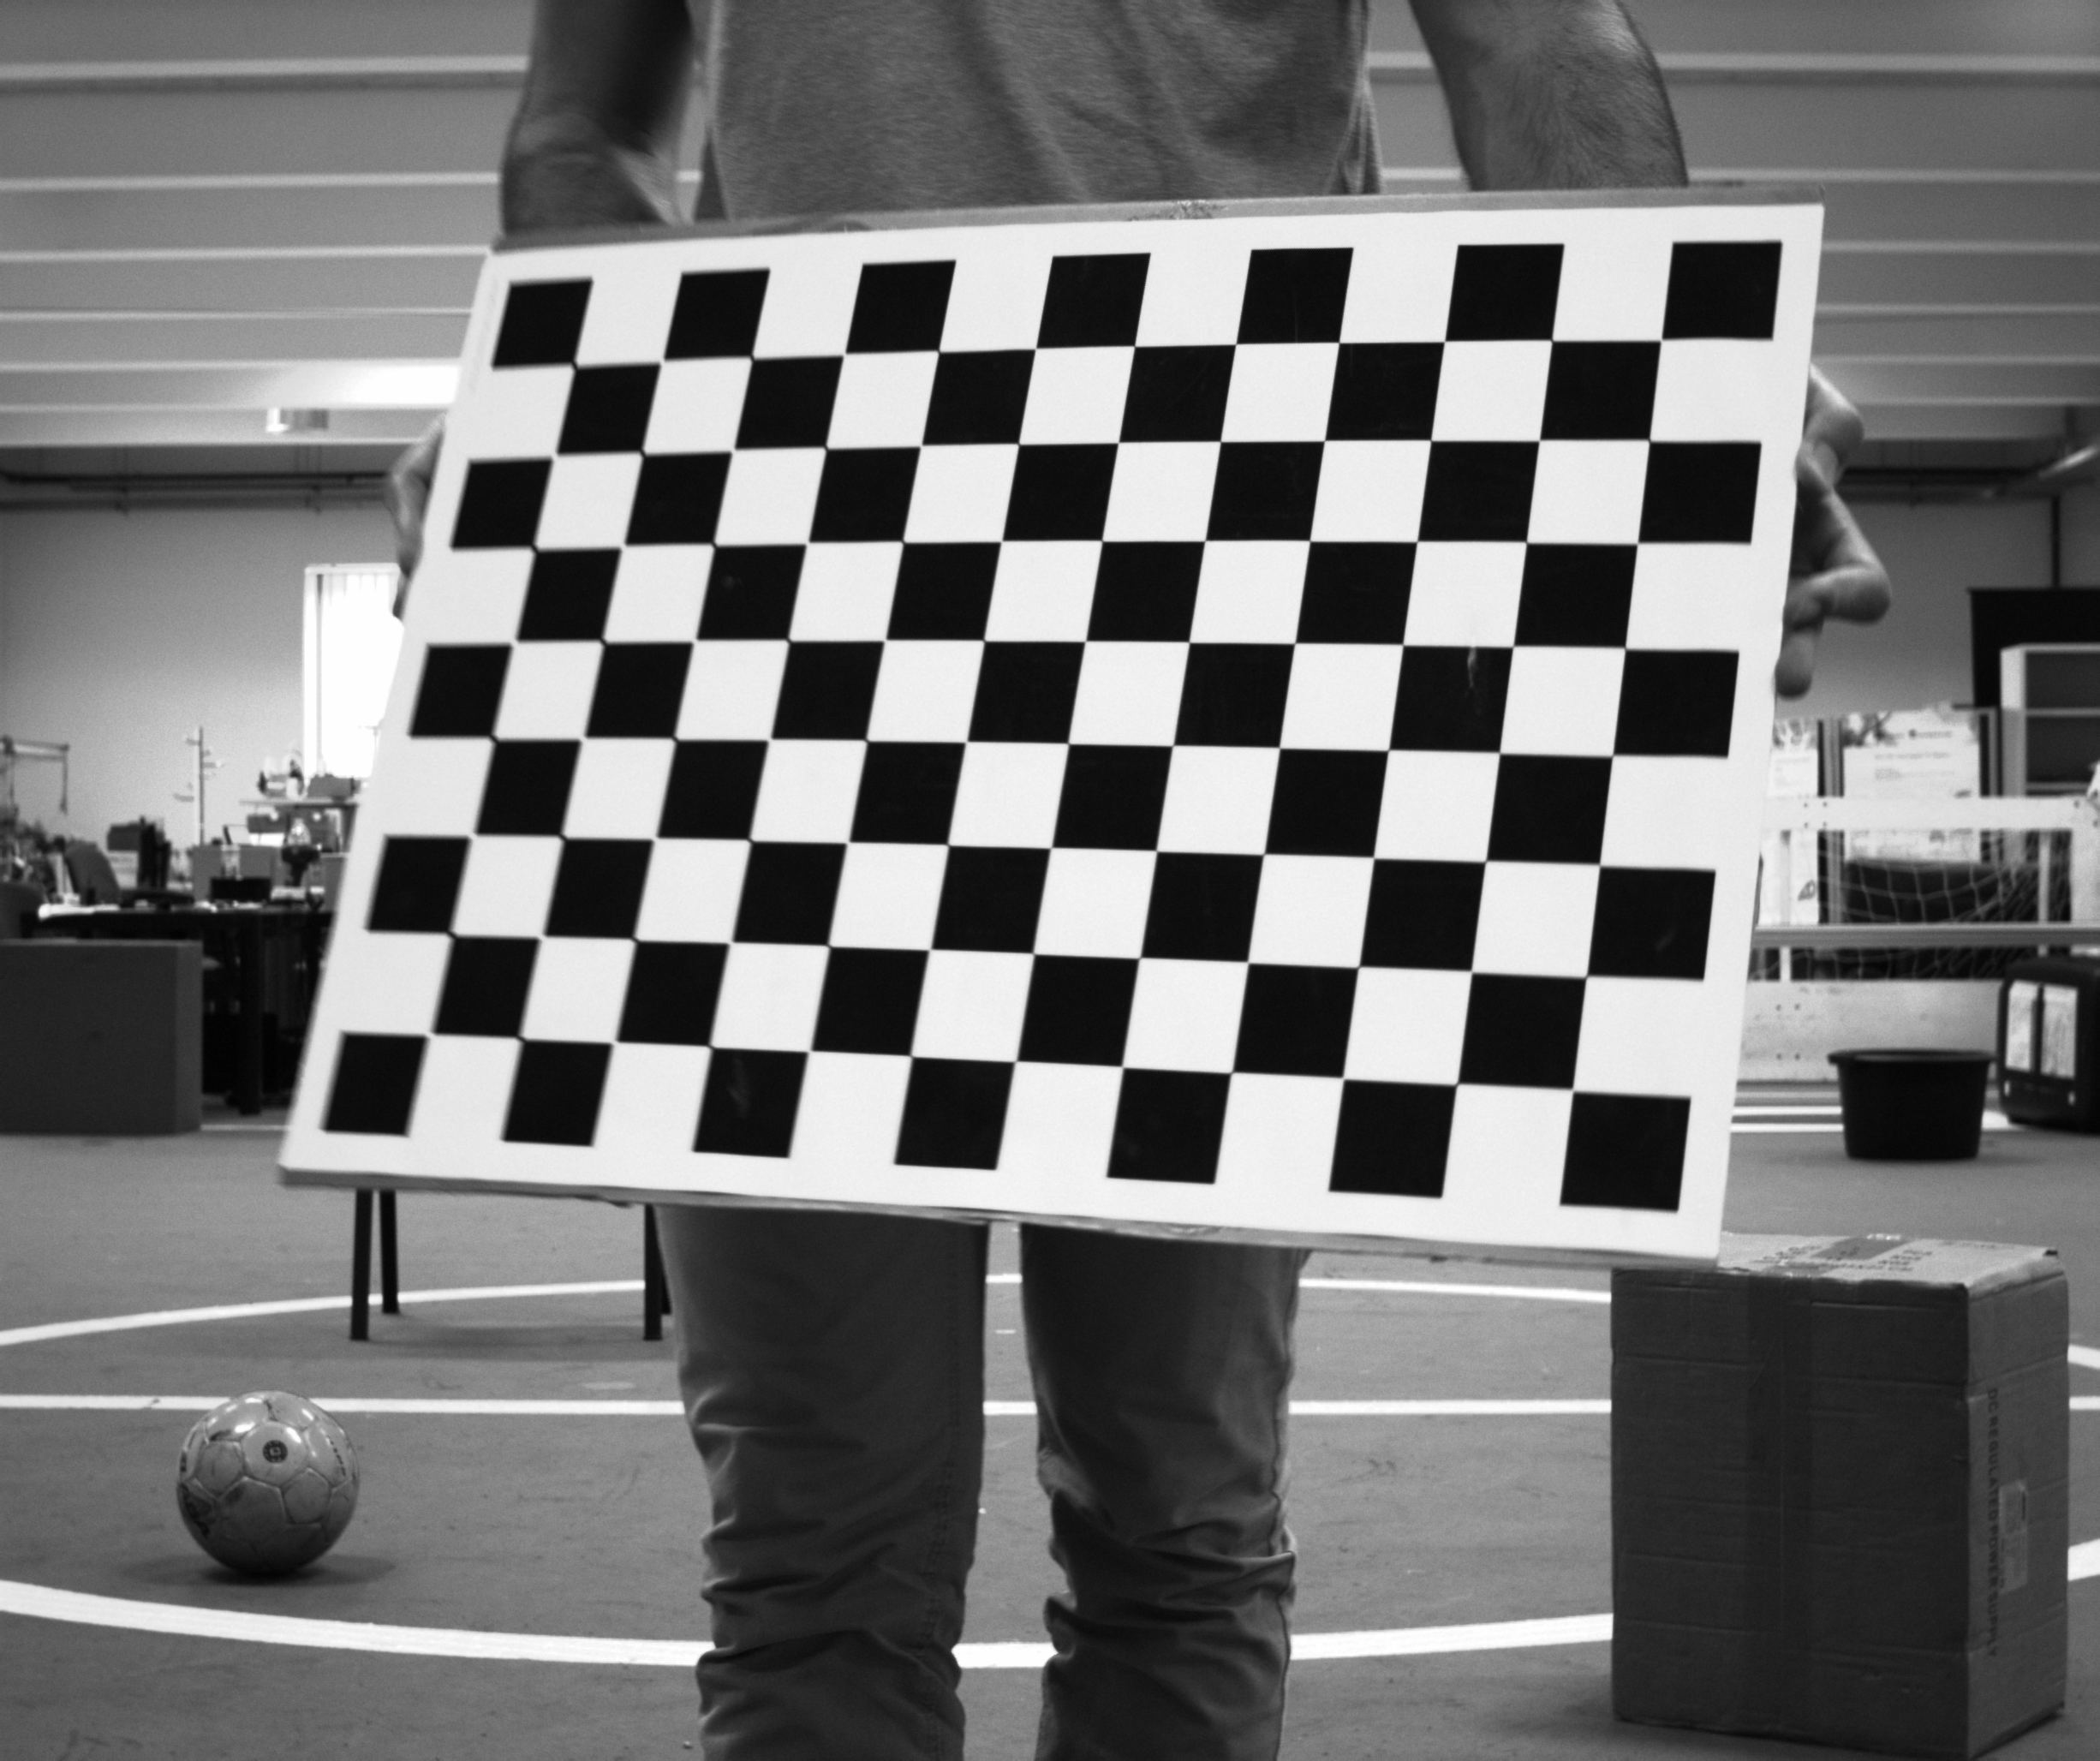
\includegraphics[width=0.9\textwidth]{img/camera-calibration/left-0030.png}
	\end{subfigure}
	\begin{subfigure}[c]{0.30\textwidth}
		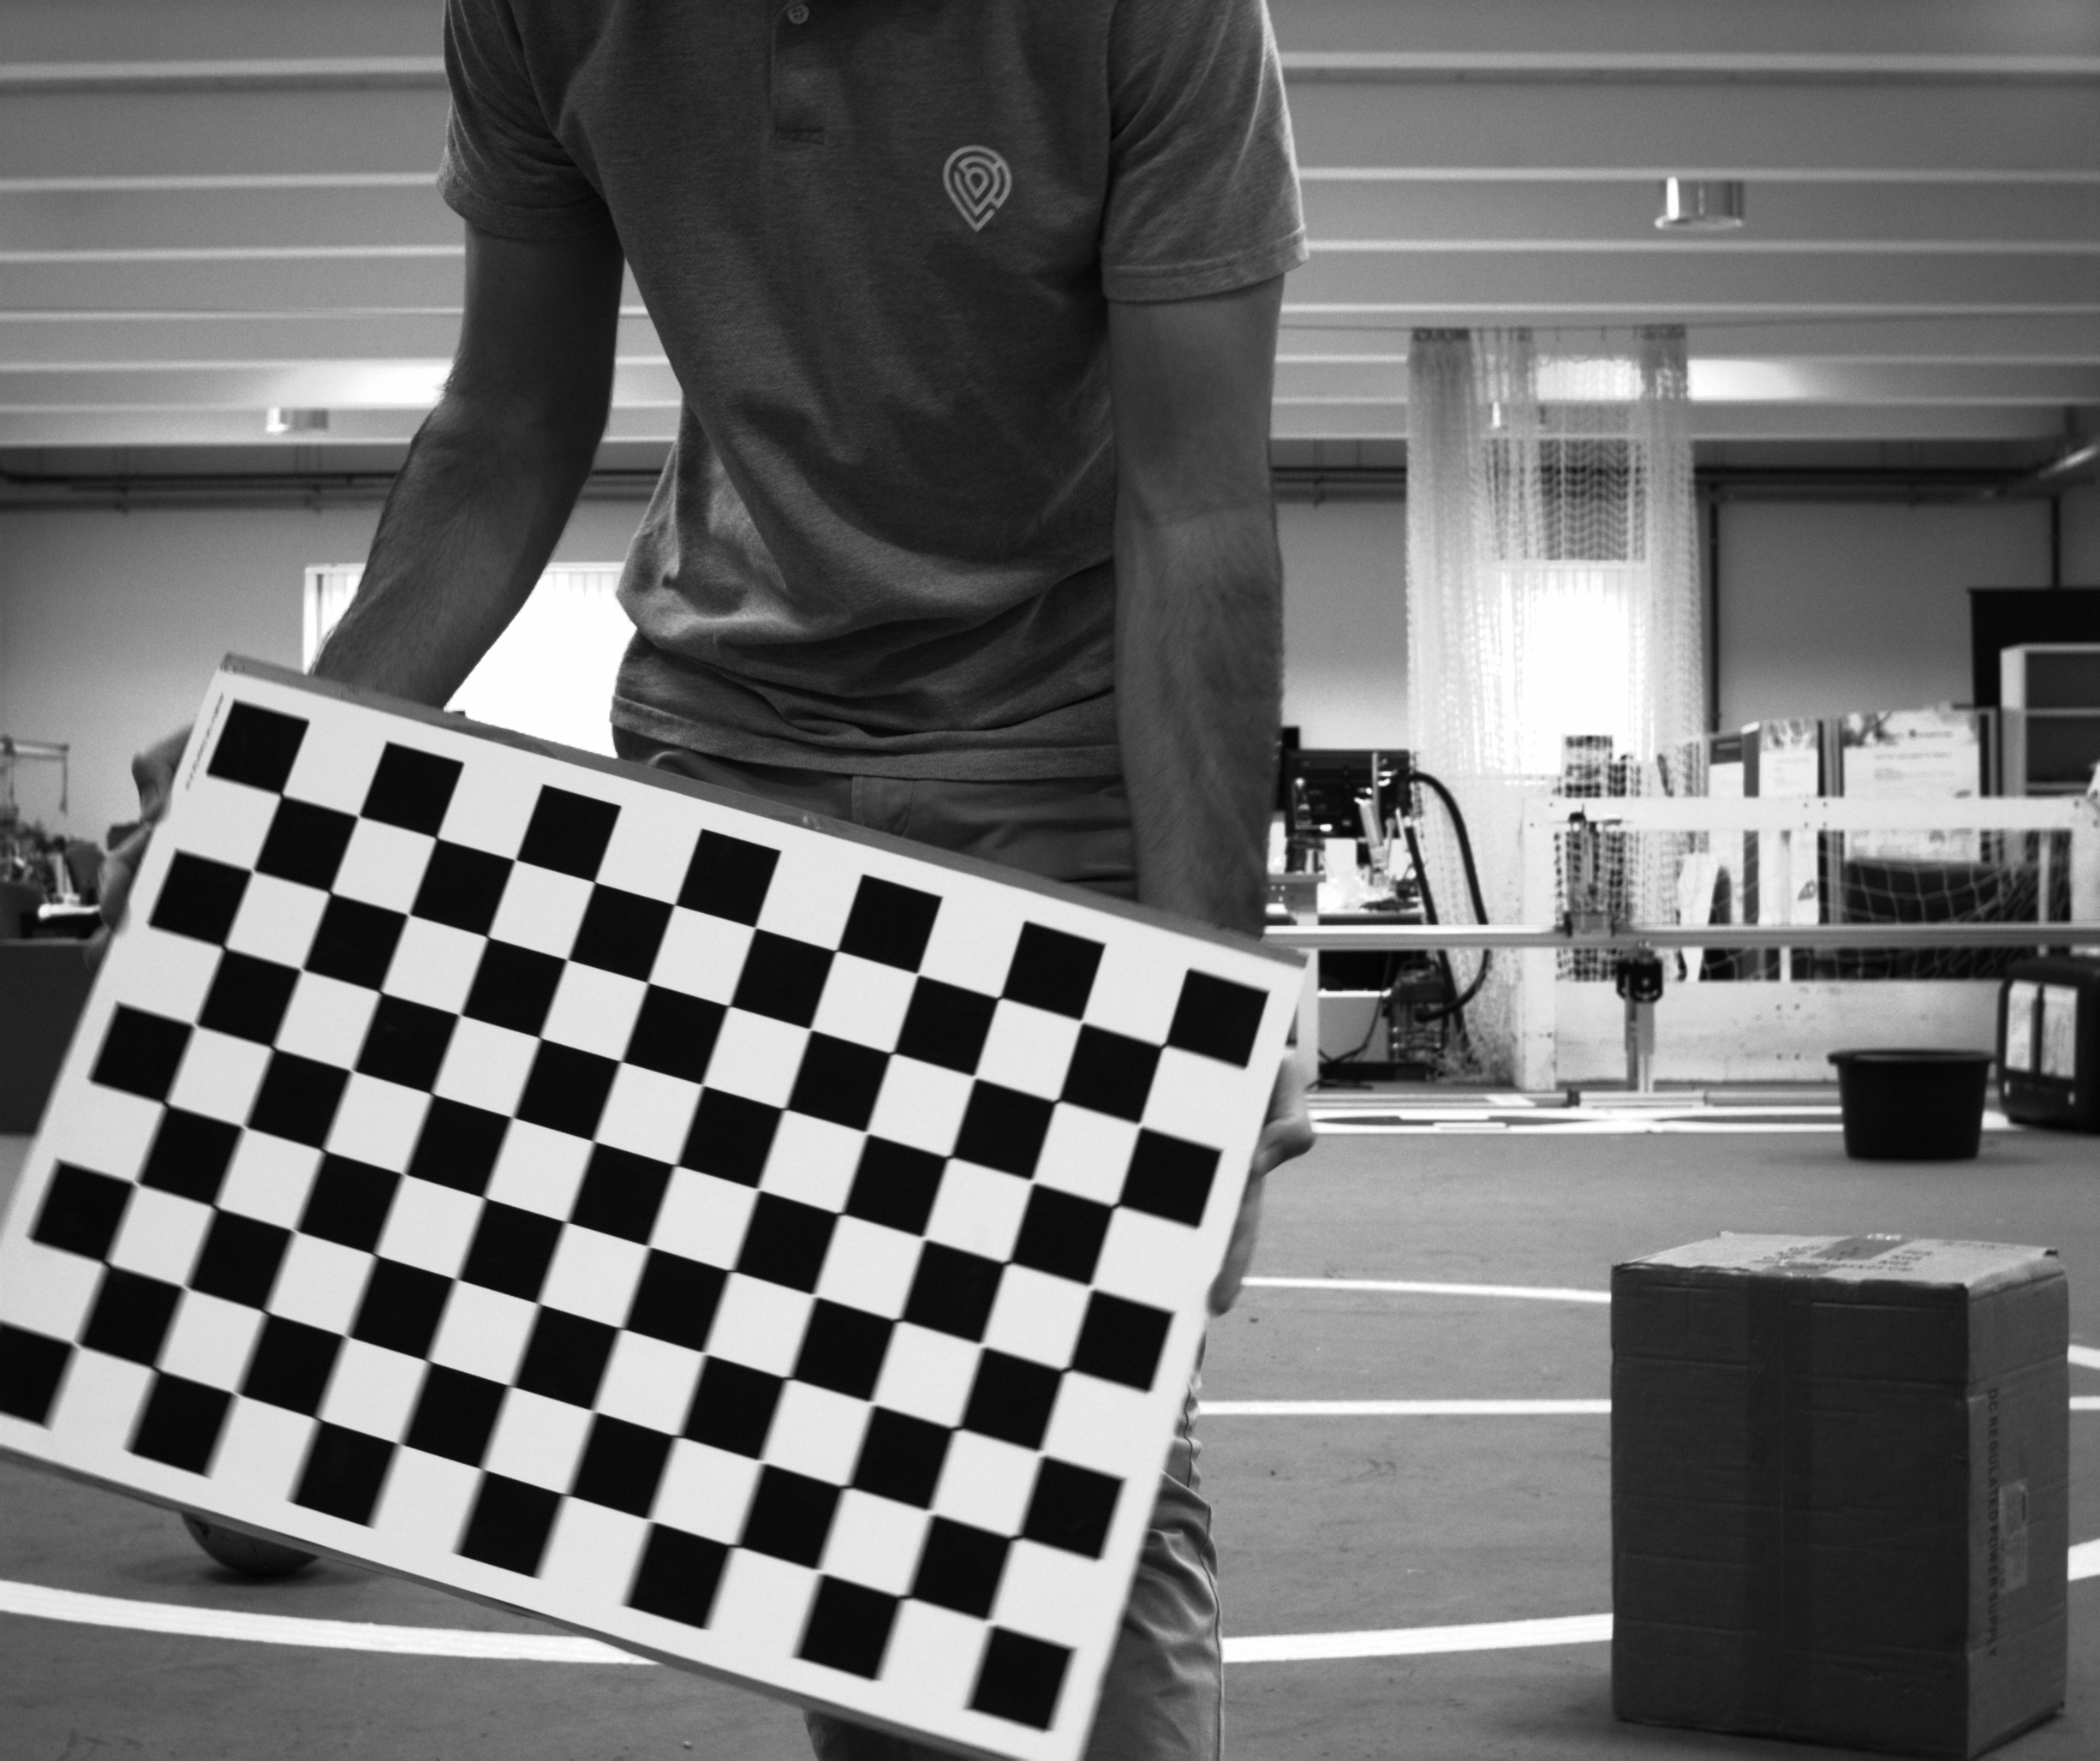
\includegraphics[width=0.9\textwidth]{img/camera-calibration/left-0044.png}
	\end{subfigure}
	\begin{subfigure}[c]{0.30\textwidth}
		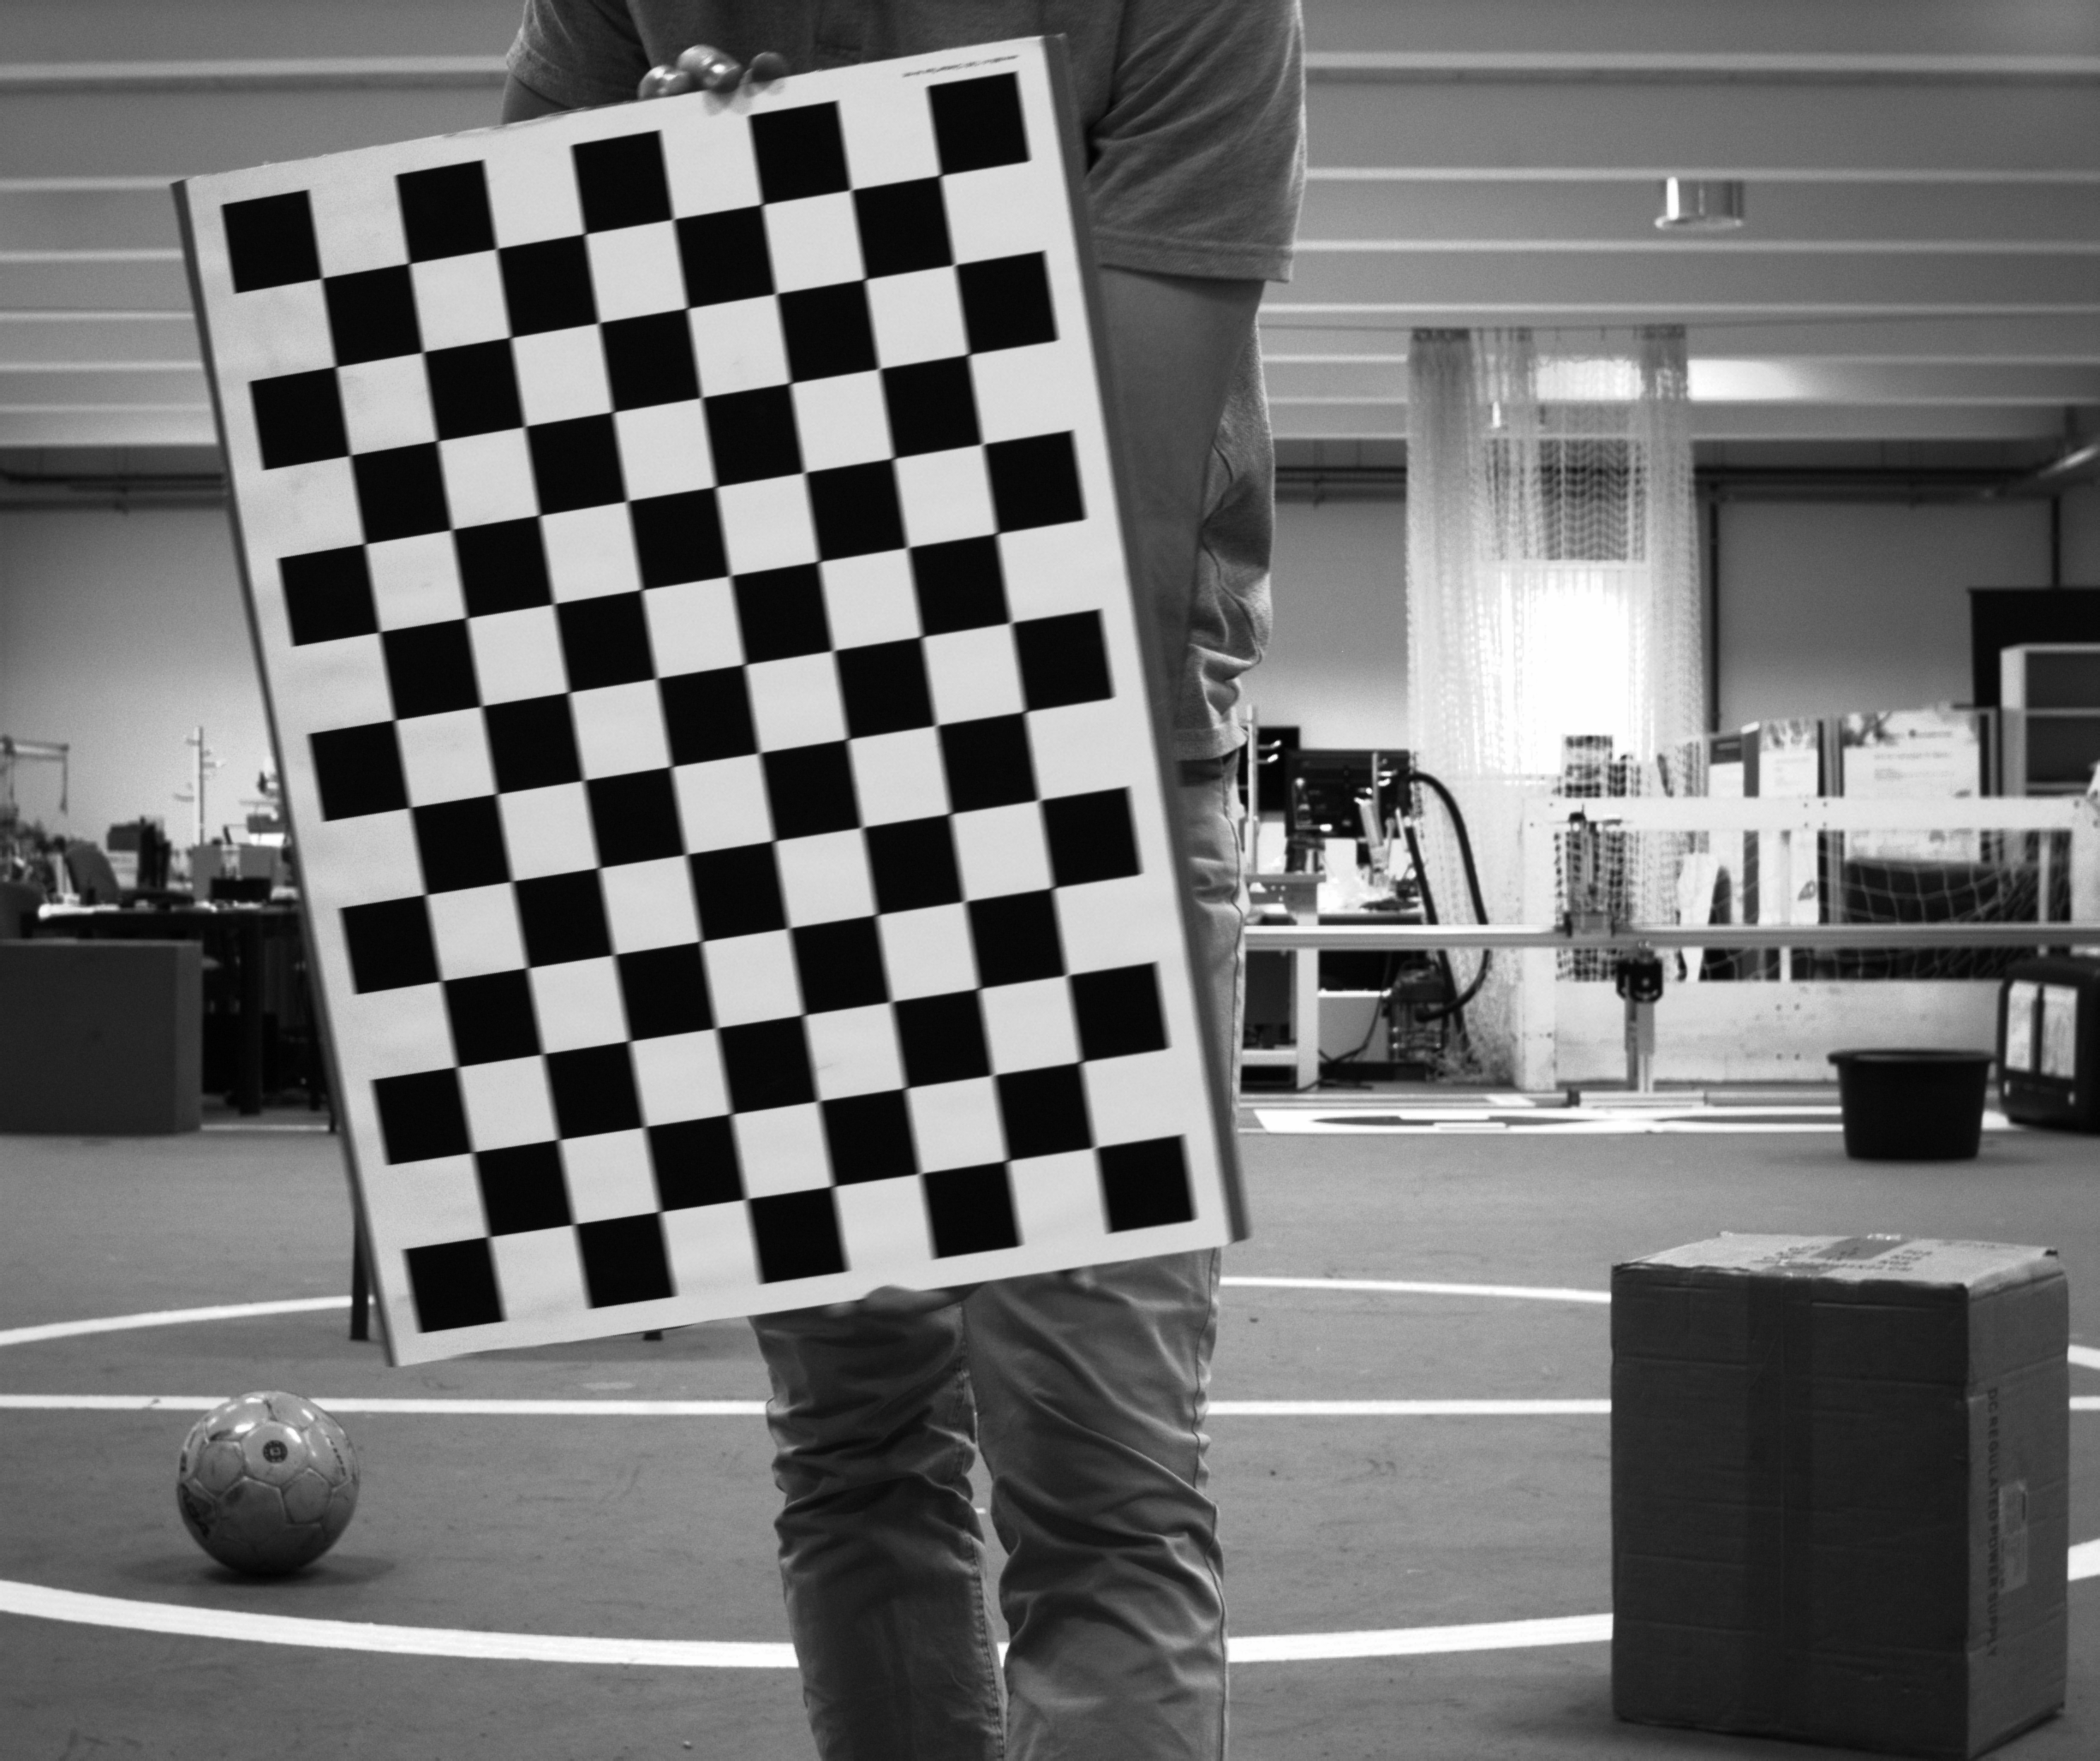
\includegraphics[width=0.9\textwidth]{img/camera-calibration/left-0048.png}
	\end{subfigure}
	
	\caption{Subset of 6 figures used on camera intrinsic calibration. The figures are all on grayscale and for each figure, the chessboard pattern was moved to generate an unique rotational matrix and translation vector in relation to the camera.}
	\label{fig:camera-calibration-images}
\end{figure}

\subsubsection{Frame Rate and Bandwith concerns}
Despite the straightforness of the process, one of the secondary goals of this thesis is to produce a dataset of scenarios on which \ac{lidar} interference is present. Such goal implies that all data must be properly recorded and stored, including calibration data. \ac{ros} provides \emph{rosbag}, a package for recording and playing back messages exchanged in a \ac{ros} network, which is used to save data on an external hard-drive.

However, preliminary tests with this tool indicate that it cannot save images topics at $9.2$~\ac{fps}. Other tests have shown that $8$~\ac{fps} is the best scenario where \emph{rosbag} can record data without causing buffer dumps due to overrun errors. 


When calibrating the camera, \emph{camera\_calibration} package drops the frame rate to 4~\ac{fps}, because it cannot accompanied the data flow. If debayrization and/or retification is being applied to the image with the intuit to save a pre-processed image, frame rate drops to 2~\ac{fps}, since \emph{image\_proc}, the package responsible for pre-processing the image, cannot process images at the data-rate required for them to be saved on disk, introducing an overhead. Therefore, all images are sent from camera on the raw format \emph{BayerGB8} and recorded in the same format. Note that despite the camera providing  the \emph{RGB8Packed} color format, the hardware processment required on the camera forces framerate to drop from $8$ \ac{fps}, reason why it was not choosed.

At 8~\ac{fps}, the bandwisth occupied by a 5~\ac{mp} image stream is equal to a: $8 \cdot 2452 \cdot 2056 \approx 40 \text{Mbytes/s}$. Manta bandwidth limit configuration register was set to a value 25\% higher, to accomodate other transmissions from the computer to camera and vice-versa: 50 Mbytes/s. No bandwith problems were registered, only occasionaly frame drops on the starting or ending of computer processes.

Therefore, for normal operation, Manta \ac{avt} G-504C is set to trigger image capture at a fixed frame rate of $8$~\ac{fps} and when being under an internal calibration procedure, at $4$~\ac{fps}. However, to run at this \ac{fps}, the camera must be able to output data at this speed, which results from other constrains.

\subsubsection{Lens Aperture and Exposure Time}
Thorlabs\cp lens has several possible apertures: $f/1.4$, $f/2.0$, $f/2.8$, $f/4.0$, $f/8.0$, $f/16.0$. The smaller the F-number\footnote{F-number represents the ratio of the lens' focal length to its diameter.}, the bigger the aperture is and wider the lens entrance is, letting more light pass to the camera sensor. More light indicates that exposure time can be reduced, since for the sensor to receive the same amount of light to produce a sharp image, less time is required.

However, decreasing the F-number reduces the Hyperfocal distance (see equation~\ref{eq:hyperfocal_distance}), which in turns reduces \acf{dof}. A tradeoff must be addressed between \ac{dof} and F-number, which implies that three parameters must be ajusted: \ac{dof}, exposure time, image \ac{fps}, since their are all interconnected. As stated above, a maximum \ac{fps} is desirable, but due to recording constraints of the \emph{rosbag} package, $8$~\ac{fps} is the desired image frame-rate. This implies that, at $8$\ac{fps}, the camera must never take more than $125ms$ since the start of exposure to the broadcast of the message on the Ethernet network, which means that exposure time must be inferior. 

Trought experimental analysis, the maximum exposure which seems to not disturbe the desired frame rate is $100ms$. Now, the F-number needs to be adjusted not only to ensure the requirements of the exposure time are met and to maximize \acl{dof}, but also to ensure that exposure can be increased or decrease to accomodate the daylight intensity variations. Such constrains results on a F-number of $f/4.0$ and an exposure time variation between 80ms to 100ms during daylight.

\subsubsection{\acl{dof} and calibration object}
Solving for equation~\ref{eq:hyperfocal_distance} and replacing it value on equation~\ref{eq:dof-subject-distance}, we cand obtain $d$, the object distance at each the camera must be focused. The object to be focused is the calibrating pattern. The $DoF_{near}$ limit is the distance at each the calibration pattern fills the camera~\ac{fov}.

\begin{subequations}
	\begin{align}
		H & = \frac{16mm^2}{4.0 \cdot 0.020mm} + 16mm  = 3.216 m \label{eq:hyperfocal-distance-value} \\
		\vspace{25mm}
		d & = \frac{(3.216 - 16mm) \cdot 1.405}{3.216 - 1.405} = 2.49m \label{eq:dof-subject-distance-value}
	\end{align}
\end{subequations}

After focusing the camera, the \emph{cameracalibrator.py} node is run, using the following command. Note that the chessboard dimensions argument is $12\times 8$ and not $13 \times 9$, because the size argument refers to the number of interior corners, not number of squares.


\begin{verbatim}
    rosrun camera_calibration cameracalibrator.py --size 12x8 --square 0.044  
        monocular:=/camera image:=/camera/image_raw
\end{verbatim}


After the \ac{gui} registers all the images, the calibration parameters calculation can be initiated and the parameters can be saved on a \textit{.ost} file for later use and/or sent the configraiton to camera. 

To interact with the Manta AVT G-504C, \emph{avt\_vimba\_camera} \ac{ros} package~\cite{AVTROSdriver}, which dependes on VIMBA GigE SDK, is used to drive the camera, and is compatible with the \emph{camera\_calibration} package. 

\subsection{Camera Calibration Results}
The \ac{ros} node diagrams can be seen on figure~\ref{fig:camera-calibration-rosgraph}. On sub-figure~\subref{fig:camera-calibration-avt-rosgraph}, the nodes and topics for the calibration procedure using the data directly from the driver are shown. Sub-figure~\subref{fig:camera-calibration-bag-rosgraph} shows the difference node graph if the data is played using the \emph{rosbag} tool.

\begin{figure}[H]
	\vspace{5mm}
	\centering
	\begin{subfigure}[c]{0.8\textwidth}
		\centering
		
\includegraphics[width=0.8\textwidth]{img/camera-calibration/bag-rosgraph.png}
		\caption{\ac{ros} node graph for the camera calibration procedure using the \emph{rosbag} tool. \emph{RosbagPlayer} is the node that plays back the data stored on the bag file.}
		\label{fig:camera-calibration-bag-rosgraph}
	\end{subfigure}
	\vspace{5mm} \\ 
	\begin{subfigure}[c]{0.8\textwidth}
		\centering
		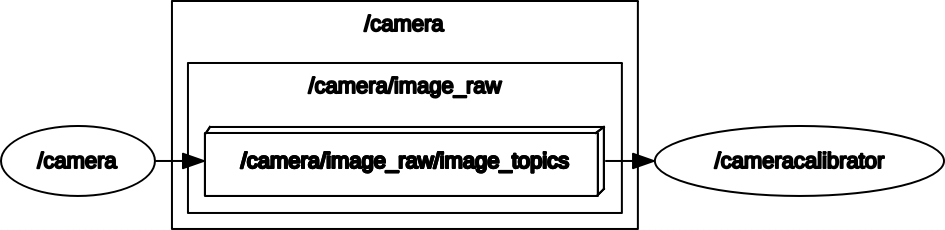
\includegraphics[width=0.8\textwidth]{img/camera-calibration/avt-rosgraph.png}		
		\caption{\ac{ros} node for the camera calibration procedure using the \ac{avt} Vimba \ac{ros} driver. \emph{camera} node refers to \ac{ros} node that wraps the \ac{avt} Vimba driver.}
		\label{fig:camera-calibration-avt-rosgraph}
	\end{subfigure}
	\caption{Camera Calibration node graph for \ac{ros} nodes. \emph{cameracalibrator} is the node responsible for computing the intrinsic camera calibration parameters, either they are comming from the camera driver~\subref{fig:camera-calibration-avt-rosgraph} or the being replayed using \emph{rosbag}~\subref{fig:camera-calibration-bag-rosgraph}.}
	\label{fig:camera-calibration-rosgraph}
\end{figure}

The camera was calibrated everyday experimental measures were taken. The calibration for one of these days is shown below, on equation~\ref{eq:camera-calibration-results}.

\begin{subequations}
	\label{eq:camera-calibration-results}
	\begin{align}
		K & = 
		\begin{bmatrix}
			4595.944192 & 0.0         &  1313.9194945 \\
			0.0         & 4593.466666 &  952.554450 \\
			0.0         & 0.0         &  1.0
		\end{bmatrix} \\
		D & = 
		\begin{bmatrix}
			-0.304037 & 1.364428 &  -0.005705 & 0.003330 & 0.000000
		\end{bmatrix} \\
		P & = 
		\begin{bmatrix}
			4529.381836 & 0.0         & 1318.010062 & 0.0 \\
			0.0         & 4534.939941 & 947.167736  & 0.0 \\
			0.0         & 0.0         & 1.0         & 0.0 
		\end{bmatrix}
	\end{align}
\end{subequations}

	

\section{\ac{lidar} Intrinsic Calibration}
Unlike a camera, \acp{lidar} does not possess a typical calibration procedure. For Velodyne VLP-16 reflectivity measurements are factory calibrated, in a procedure described in~\cite{vlp16} and a \ac{xml} file is provided with the \ac{lidar}, which contain offset parameters for the polar angles of each laser.

This file is must be converted to a more suitable format, \acs{yaml}~\footnote{\acs{yaml} is an acrononym for \acl{yaml}. The author chose not to expand such  ``peculiar'' acronym on the text to facilitate reading.}, which is \ac{ros} default and can be loaded by the Velodyne \ac{ros} driver package, \emph{velodyne}, for correction of the \ac{lidar} measurements. After observing the point cloud with tests objects such as boxes and walls, this calibration is concluded to be accurate and no further procedures were necessary.

\section{Camera and \ac{lidar} Extrinsic Calibration}

